\documentclass[twoside,openright,final]{bhamthesis}

\usepackage[utf8]{inputenc}

\usepackage{amssymb}
\usepackage{amsmath}
\usepackage{bm}
\newcommand{\mb}[1]{\({#1}\)}

\usepackage{amsthm}
\usepackage[english]{babel}

\usepackage{listings}
\makeatletter % making underscore larger in listings
\DeclareTextCommandDefault{\textunderscore}{%
  \leavevmode\kern0.03em\vbox{\hrule\@width.6em \@height-.25ex \@depth0.37ex}\kern0.03em}
\makeatother
\newcommand{\hyphen}{\operatorname{-}} % making hypen smaller in math-mode
\def\Plus{\texttt{+}}
\makeatletter
\newsavebox{\@brx}
\newcommand{\llangle}[1][]{\savebox{\@brx}{\(\m@th{#1\langle}\)}%
  \mathopen{\copy\@brx\kern-0.5\wd\@brx\usebox{\@brx}}}
\newcommand{\rrangle}[1][]{\savebox{\@brx}{\(\m@th{#1\rangle}\)}%
  \mathclose{\copy\@brx\kern-0.5\wd\@brx\usebox{\@brx}}}
\makeatother

\usepackage{geometry}

\usepackage{graphicx}
\graphicspath{ {images/} }

%\usepackage{indentfirst}

\usepackage{enumerate,letltxmacro}
\usepackage{enumitem}
%\LetLtxMacro\itemold\item
%\renewcommand{\item}{\itemindent0.5cm\itemold} % set indentation for items
\usepackage{hyperref}
\hypersetup{
    colorlinks,
    citecolor=black,
    filecolor=black,
    linkcolor=black,
    urlcolor=black
}

\usepackage{etoolbox} % set reference header to null
\patchcmd{\thebibliography}{\section*{\refname}}{}{}{}

\usepackage{cite}


% ---- Set page style ---- %
\pagestyle{plain}

% I don't know what it does really
%\newcommand*{\approxident}{%
%  \mathrel{\vcenter{\offinterlineskip
%  \hbox{$\sim$}\vskip-.35ex\hbox{$\sim$}\vskip-.35ex\hbox{$\sim$}}}}

% setting odd/even pages margin
%\setlength{\textheight}{21cm} % Height of the main body of the text
%\setlength{\topmargin}{0cm} % 1'' margin on top of page
%\setlength{\headsep}{1.5cm}  % space between header and top of body
%\addtolength{\headsep}{-\headheight} % See The LaTeX Companion, p 85
%\setlength{\footskip}{1cm}  % space between footer and bottom of body
%\setlength{\textwidth}{14cm} % width of the body of the text
\setlength{\oddsidemargin}{1cm} % 2cm margin on the left for odd pages
\setlength{\evensidemargin}{0.5cm} % 2cm margin on the right for even % pages

\title{\textbf{Validated Parsing of Regular Expressions in Agda}}
\department{Computer Science}
\degree{BSc. Computer Science}
\author{Wai Tak, Cheung}
\studentid{1465388}
\supervisor{Dr. Martín Escardó}

\begin{document}
\maketitle


\abstract
\par In this project, we intend to study the feasibility of
constructing a certified translation algorithm of regular expressions to finite automata in Type
Theory. The translation consists of several steps: regular expressions
to \(\epsilon\)-NFA using Thompson's
construction; \(\epsilon\)-NFA to NFA by removing
\(\epsilon\)-transitions; DFA to DFA by powerset construction; and DFA
to MDFA by removing unreachable states and quotient construction. The
correctness of the translation is obtained by
showing that their accepting languages are equal. The above
translation and its correctness proofs are formalised in Agda -- a
dependently-typed functional programming language based on Type Theory. 
\\ \\
Keywords: regular expression, finite automata, type theory, agda

\acknowledgments
\par I would like to express my greatest appreciation to Dr. Martín
Escardó, my project supervisor, for his patient guidance, enthusiastic
encouragement and valuable advises on this project. 

\repository
\vspace{7cm}
\begin{center}
  All software for this project can be found at \\
  https://codex.cs.bham.ac.uk/svn/projects/2015/wtc488/
\end{center}

\chapter*{List of Abbreviations}
\addcontentsline{toc}{chapter}{List of Abbreviations}
\let\cleardoublepage\clearpage
\begin{tabular}{ll}
  \textbf{\(\epsilon\)-NFA} & Non-deterministic Finite Automaton with
                              \(\epsilon\)-transition \\
  \textbf{NFA} & Non-deterministic Finite Automaton \\
  \textbf{DFA} & Deterministic Finite Automaton \\
  \textbf{RDFA} & Deterministic Finite Automaton in which all its states are
                  Reachable \\
  \textbf{MDFA} & Minimised Deterministic Finite Automaton
\end{tabular}

%\setcounter{tocdepth}{3}
\tableofcontents

\section{Introduction}
\par This project aims to study the feasibility of formalising
Automata Theory \cite{aho1972} in Type Theory \cite{martin1984}. 
... [ small intro to type theory? type theory and proof assistant and
dependent types -> Agda will be used ] 

\par Automata Theory is an extensive work; therefore, it will be unrealistic to
include all the materials under the time constraints. Accordingly,
this project will only focus on the theorems and
proofs that are related to the translation of regular expressions
to finite automata. In addition, this project also serves as an
example on how complex and non-trivial proofs are formalised. 

\par Our Agda formalisation consists of two components: 1) the
translation of regular expressions to DFA and 2)
the correctness proofs of the translation. At this stage, we are only
interested in the correctness of the translation but not the
efficiency of the algorithms. 


\subsection{Motivation}
\par My motivation on this project is to learn and apply
dependent types in formalising programming logic. At the beginning, I
was new to dependent types and proof assistants. Therefore, we
had to choose carefully what theorems to formalise. On one hand, the theorems
should be non-trivial enough such that a substantial amount of work is required
to be done. On the other hand, the theorems should not be too
difficult because I am only a beginner in this area. Finally, we
decided to go with the Automata Theory as its basic concepts were
explained in the course \textit{Model of Computation}. 


\subsection{Outline}
\par Section 2 will be a brief introduction on Agda and
dependent types. We will describe how Agda can be used as a proof
assistant by giving examples of formalised proofs. Experienced Agda
users can skip this section and start from section 3 directly. In
section 3, we will describe several researches
that are also related to the formalisation of Automata
Theory. Following the background, section 4 will be a detail description of our
work. We will walk through the two components of our Agda
formalisation. Note that the definitions,
theorems and proofs written in this section are extracted from our
Agda code. They may be different from
their usual mathematical forms in order to adapt to the environment of
Type Theory. In section 5, we will discuss two possible extensions
to our project: 1) Myhill-Nerode Theorem and 2) the Pumping
Lemma. After that, in section 6, we will evaluate the project as a
whole. Finally, the conclusions will be drawn. 

\section{Agda}
\par Agda is a dependently-typed functional programming language and a
proof assistant based on Intuitionistic Type Theory
\cite{martin1984}. The current version (Agda 2) is rewritten by Norell
\cite{norell2007} during his doctorate study at the Chalmers University of
Technology. In this section, we will describe the basic features of
Agda and how dependent types are employed to construct programs and
proofs. Most of the materials presented below can also be
found in the two tutorial papers \cite{bove2009} and
\cite{norell2009}. Interested readers can read the two papers in order to get
a more precise idea on how to work with Agda. Now, we will begin by
showing how to do ordinary functional programming in Agda. 


\subsection{Simply Typed Functional Programming}
\par Haskell is the implementation language
of Agda, as shown below, Agda has borrowed many features from
Haskell. In the following paragraphs, we will demonstrate how to
define basic data types and functions. 

\paragraph{Boolean} We first declare the type of Boolean values in Agda.  
\begin{lstlisting}[mathescape=true,xleftmargin=.3\textwidth]
data Bool : Set where
  true  : Bool
  false : Bool
\end{lstlisting}

\par \mb{Bool} has two
constructors: \mb{true} and \mb{false}. These two constructors
are also elements of \mb{Bool} as they take no arguments. On
the other hand, \mb{Bool} itself is a member of the type
\mb{Set}. The type of \mb{Set} is \mb{Set_1} and the type of \mb{Set_1} is
\mb{Set_2}. The type hierarchy goes on and becomes infinite. Now, let
us define the negation of Boolean values. 
\begin{lstlisting}[mathescape=true,xleftmargin=.3\textwidth]
not : Bool $\to$ Bool
not true  = false
not false = true
\end{lstlisting}

\par Unlike in Haskell, a type signature must be provided explicitly for every
function and all possible cases must be included in the function body
while pattern matching. For instance, the function below will be rejected
by the Agda compiler as the case \mb{(not\ false)} is missing. 
\begin{lstlisting}[mathescape=true,xleftmargin=.3\textwidth]
not : Bool $\to$ Bool
not true  = false
\end{lstlisting}

\paragraph{Natural Number} Now, let us declare the type of natural
numbers in Peano style. 
\begin{lstlisting}[mathescape=true,xleftmargin=.3\textwidth]
data $\mathbb N$ : Set where
  zero : $\mathbb N$
  suc  : $\mathbb N$ $\to$ $\mathbb N$
\end{lstlisting} 

\par The constructor \mb{suc} represents the successor of a given
natural number. For instance, the number \mb{1} is equivalent to
(\mb{suc\ zero}). Now, let us define the addition of natural numbers recursively as follow:
\begin{lstlisting}[mathescape=true,xleftmargin=.3\textwidth]
_+_ : $\mathbb N$ $\to$ $\mathbb N$ $\to$ $\mathbb N$: Set where
zero + m = m
(suc n) + m = suc (n + m)
\end{lstlisting} 

\paragraph{Parameterised Types} In Haskell, the type of list \mb{[a]} is parameterised by the type
parameter \mb{a}. The analogous data type in Agda is defined as follow:
\begin{lstlisting}[mathescape=true,xleftmargin=.3\textwidth]
data List (A : Set) : Set where
  []   : List A
  _::_ : A $\to$ List A $\to$ List A
\end{lstlisting} 

\par Let us try to define a function which takes a
list as the argument and returns the first element of the list. 
\begin{lstlisting}[mathescape=true,xleftmargin=.3\textwidth]
head : {A : Set} $\to$ List A $\to$ A
head [] = {!!}
head (x :: xs) = x
\end{lstlisting} 

\par What should be returned in case \mb{[\ ]}? In Haskell, the \mb{[\
  ]} case can simply be skipped and an error will be produced by the
compiler. However, as we have mentioned
before, the function body must contains all the possible cases. One
possible workaround is to return \mb{nothing} of the \mb{Maybe} type
for case \mb{[\ ]}. Another solution is
to constrain the arguments using dependent types such that the input list will always have at least one element. 


\subsection{Dependent Types}
\par A dependent type is a type that depends on values of other
types. For example, \mb{A^n} is a vector that contains \mb{n} elements
of \mb{A}. These kind of types is not possible
to be declared in simply-typed systems like Haskell\footnotemark and Ocaml. Now, let
us look at how it is declared in Agda.
\footnotetext{Haskell itself does not support dependent types by
  its own. However, there are several APIs in Haskell that simulates
  dependent types, for example, Ivor \cite{ivor2016} and
  GADT.}
\begin{lstlisting}[mathescape=true,xleftmargin=.3\textwidth]
data Vec (A : Set) : $\mathbb N$ $\to$ Set where
  []   : Vec A zero
  _::_ : $\forall$ {n} $\to$ A $\to$ Vec A n $\to$ Vec A (suc n)
\end{lstlisting} 

\par In the type signature, (\mb{A : Set}) is the type
parameter while \mb{\mathbb N \to Set} means
that \mb{Vec} takes a number \mb{n} from \mb{\mathbb N} and produces a
type that depends on \mb{n}. Different types will be produced by giving different natural
numbers to the inductive family \mb{Vec}. For example, \mb{Vec\ A\ zero} is
the type of empty vectors and \mb{Vec\ A\ 10} is another vector type with length ten. 

\par Dependent types allow us to be more
expressive and precise over type declaration. Let us declare the
\mb{head} function for \mb{Vec}. 
\begin{lstlisting}[mathescape=true,xleftmargin=.3\textwidth]
head : {A : Set}{n : $\mathbb N$} $\to$ Vec A (suc n) $\to$ A
head (x :: xs) = x 
\end{lstlisting} 

\par Only the (\mb{x :: xs}) case needs to be pattern matched because
the type \mb{Vec\ A\ (suc\ n)} ensures that the argument will never
be \mb{[\ ]}. Apart from vectors, a type of binary
search tree can also be declared in which any tree of this type is guaranteed to be
sorted. However, this is not our major concern and thus we will not be
looking into it. Interested readers can take a look at 
Section 6 in \cite{bove2009}. Furthermore, dependent types also allow
us to encode predicate logic and program specifications as
types. These two applications will be describe in later part and now,
we will first discuss the idea of propositions as types. 


\subsection{Propositions as Types}
\par In the 1930s, Curry identified the
correspondence between propositions in propositional logic and types
\cite{curry1934}. After that, in the 1960s, de Bruijn and Howard extended
Curry's correspondence to predicate logic by introducing dependent
types \cite{bruijn1968, howard1969}. Later on, Martin-L\"of published
his work, Intuitionistic Type Theory \cite{martin1984}, which turned the correspondence into a new
foundational system for constructive mathematics. 

\par In the paragraphs below, we will show how the correspondence is
formalised in Agda. Note that Intuitionistic Type
Theory is based on constructive logic but not classical logic and there
is a fundamental difference between them. Interested readers can take a look at
\cite{avigad2000}. Now, we will begin with propositional logic. 

\subsubsection{Propositional Logic} 
\par In general, Curry's correspondence
states that a proposition can be interpreted as a set of its proofs. A
proposition is true if and only if its set of proofs is inhabited,
i.e. there is at least one element in the set; it is false if and only
if its set of proofs is empty. 

\paragraph{Truth} For a proposition to be always true, its
corresponding type must have at least one element. 
\begin{lstlisting}[mathescape=true,xleftmargin=.3\textwidth]
data $\top$ : Set where
  tt : $\top$
\end{lstlisting} 

\paragraph{Falsehood} The proposition that is always
false corresponds to a type having no elements at all. 
\begin{lstlisting}[mathescape=true,xleftmargin=.3\textwidth]
data $\bot$ : Set where
\end{lstlisting} 

\paragraph{Conjunction} Suppose \mb{A} and \mb{B} are propositions, then the
proofs of their conjunction \mb{A \wedge B} should contain both a proof of \mb{A} and a proof
of \mb{B}. In Type Theory, it corresponds
to the product type. 
\begin{lstlisting}[mathescape=true,xleftmargin=.3\textwidth]
data _$\times$_ (A B : Set) : Set where
  _,_ : A $\to$ B $\to$ A $\times$ B
\end{lstlisting} 

\par The above construction resembles the introduction rule of
conjunction while the elimination rules are formalised as follow:
\begin{lstlisting}[mathescape=true,xleftmargin=.3\textwidth]
fst : {A B : Set} $\to$ A $\times$ B $\to$ A
fst (a , b) = a

snd : {A B : Set} $\to$ A $\times$ B $\to$ B
snd (a , b) = b
\end{lstlisting} 


\paragraph{Disjunction} Suppose \mb{A} and \mb{B} are propositions, then the
proofs of their disjunction \mb{A \vee B} should contains either a proof of \mb{A} or a
proof of \mb{B}. In Type Theory, it is represented by the sum type. 
\begin{lstlisting}[mathescape=true,xleftmargin=.3\textwidth]
data _$\uplus$_ (A B : Set) : Set where
  inj$_1$ : A $\to$ A $\uplus$ B
  inj$_2$ : B $\to$ A $\uplus$ B
\end{lstlisting} 

\par The elimination rule of disjunction is defined as follow: 
\begin{lstlisting}[mathescape=true,xleftmargin=.3\textwidth]
$\uplus \hyphen$elim : {A B C : Set} 
         $\to$ A $\uplus$ B 
         $\to$ (A $\to$ C) 
         $\to$ (B $\to$ C) 
         $\to$ C
$\uplus \hyphen$elim (inj$_1$ a) f g = f a
$\uplus \hyphen$elim (inj$_2$ b) f g = g b
\end{lstlisting} 

\paragraph{Negation} Suppose \mb{A} is a proposition, then its negation is
defined as a function that transforms any arbitrary proof of \mb{A} into
the falsehood (\mb{\bot}). 
\begin{lstlisting}[mathescape=true,xleftmargin=.3\textwidth]
$\neg$ : Set $\to$ Set
$\neg$ A = A $\to$ $\bot$
\end{lstlisting} 


\paragraph{Implication} We say that \mb{A} implies \mb{B} if and only
if every proof of \mb{A} can be transformed into a proof of \mb{B}. In Type
Theory, it corresponds to a function from \mb{A} to \mb{B}, i.e. \mb{A \to
B}. 

\paragraph{Equivalence} Two propositions \mb{A} and
\mb{B} are equivalent if and only if \mb{A} implies \mb{B} and \mb{B} implies
\mb{A}. It can be considered as a conjunction of the two implications.
\begin{lstlisting}[mathescape=true,xleftmargin=.3\textwidth]
_$\iff$_ : Set $\to$ Set $\to$ Set
A $\iff$ B = (A $\to$ B) $\times$ (B $\to$ A)
\end{lstlisting} 

\paragraph{} Now, by using the above constructions, we can formalise
 theorems of propositional logic in Agda. For example, we can prove that if \mb{P} implies \mb{Q} and
\mb{Q} implies \mb{R}, then \mb{P} implies \mb{R}. 
\begin{lstlisting}[mathescape=true,xleftmargin=.3\textwidth]
prop-lem : {P Q : Set} 
           $\to$ (P $\to$ Q) 
           $\to$ (Q $\to$ R) 
           $\to$ (P $\to$ R)
prop-lem f g = $\lambda$ p $\to$ g (f p)
\end{lstlisting} 

\par By completing the function, we have provided an element
to the type \mb{(P \to Q) \to (Q \to R) \to (P \to R)} and thus, we have
also proved the theorem to be true. 


\subsubsection{Predicate Logic} 
\par We will now move on to predicate logic and
introduce the universal (\mb{\forall}) and existential (\mb{\exists})
quantifiers. A predicate is represented by a dependent type in the
form of \mb{A \to Set}. For example, we can
define the predicate of even numbers and odd numbers inductively as follow:
\begin{lstlisting}[mathescape=true,xleftmargin=.3\textwidth]
mutual
  data _isEven : $\mathbb N$ $\to$ Set where
    base : zero isEven
    step : $\forall$ n $\to$ n isOdd $\to$ (suc n) isEven

  data _isOdd : $\mathbb N$ $\to$ Set where
    step : $\forall$ n $\to$ n isEven $\to$ (suc n) isOdd
\end{lstlisting} 

\paragraph{Universal Quantifier} The interpretation of the universal quantifier is similar to
implication. In order for \mb{\forall x\in A.\ B(x)} to be true, every
proof \mb{(a)} of \mb{A} must be transformed into a proof of the predicate
\mb{B[x:=a]}. In Type Theory, it is represented by the function \mb{(x :
A) \to B\ x}. For example, we can prove by induction that for every natural
number, it is either even or odd.
\begin{lstlisting}[mathescape=true,xleftmargin=.3\textwidth]
lem$_1$ : $\forall$ n $\to$ n isEven $\uplus$ n isOdd
lem$_1$ zero = inj$_1$ base
lem$_1$ (suc n) with lem$_1$ n
... | inj$_1$ nIsEven = inj$_2$ (step n nIsEven)
... | inj$_2$ nIsOdd = inj$_1$ (step n nIsOdd)
\end{lstlisting} 

\paragraph{Existential Quantifier} The interpretation of the
existential quantifier is similar to conjunction. In order for
\mb{\exists x\in A.\ B(x)} to be true, a proof
\mb{(a)} of \mb{A} and a proof \mb{(p)} of the predicate
\mb{B[x:=a]} must be provided. In Type Theory, it is represented by the generalised
product type \mb{\Sigma}. 
\begin{lstlisting}[mathescape=true,xleftmargin=.3\textwidth]
data $\Sigma$ (A : Set) (B : A $\to$ Set) : where
  _,_ : (a : A) $\to$ B a $\to$ $\Sigma$ A B
\end{lstlisting}
\par For simplicity, we will change the syntax of \mb{\Sigma} to
\mb{\exists [ x \in A ]\ B}. As an example, we can prove that
there exists a natural number which is even. 
\begin{lstlisting}[mathescape=true,xleftmargin=.3\textwidth]
lem$_2$ : $\exists$[ n $\in$ $\mathbb N$ ] (n isEven)
lem$_2$ = zero , base
\end{lstlisting}


\subsubsection{Decidability} 
\par A proposition \mb{P} is decidable if and only if there
exists an algorithm that can decide whether it is true or false. It is
defined as follow: 
\begin{lstlisting}[mathescape=true,xleftmargin=.3\textwidth]
data Dec (A : Set) : Set where
  yes : A $\to$ Dec A
  no  : $\neg$ A $\to$ Dec A
\end{lstlisting}

\par For example, we can prove that the predicate of even numbers is
decidable. Interested readers can try and complete the proofs. 
\begin{lstlisting}[mathescape=true,xleftmargin=.3\textwidth]
lem$_3$ : $\forall$ n $\to$ $\neg$ (n isEven $\times$ n isOdd)
lem$_3$ = ?

lem$_4$ : $\forall$ n $\to$ n isEven $\to$ $\neg$ ((suc n) isEven)
lem$_4$ = ?

lem$_5$ : $\forall$ n $\to$ $\neg$ (n isEven) $\to$ (suc n) isEven
lem$_5$ = ?

even-dec : $\forall$ n $\to$ Dec (n isEven)
even-dec zero = yes base
even-dec (suc n) with even-dec n
... | yes nIsEven = no (lem$_4$ n nIsEven)
... | no $\neg$nIsEven = yes (lem$_5$ n $\neg$nIsEven)
\end{lstlisting}


\subsubsection{Propositional Equality} 
\par One important feature of Type Theory is
that the equality of propositions can also be defined as types. The
equality relation is interpreted as follow:
\begin{lstlisting}[mathescape=true,xleftmargin=.3\textwidth]
data _$\equiv$_ {A : Set} (x : A) : A $\to$ Set where
  refl : x $\equiv$ x
\end{lstlisting}

\par This states that for any \mb{x} in \mb{A}, \mb{refl} is an
element of the type \mb{x \equiv x}. More generally, \mb{refl} is a
proof of \mb{x \equiv x'} provided that \mb{x} and \mb{x'} is the same
after normalisation. For example, we can prove that \mb{\exists n\in
\mathbb N .\ n = 1 + 1} as follow:
\begin{lstlisting}[mathescape=true,xleftmargin=.3\textwidth]
lem$_3$ : $\exists$[ n $\in$ $\mathbb N$ ] n $\equiv$ (1 + 1)
lem$_3$ = suc (suc zero) , refl
\end{lstlisting}

\par We can put \mb{refl} in the proof only because both
\mb{suc\ (suc\ zero)} and \mb{1 + 1} have the same form after
normalisation. Now, let us define the elimination rule of
equality. The rule should allow us to substitute equivalence objects
into any proposition. 
\begin{lstlisting}[mathescape=true,xleftmargin=.3\textwidth]
subst : {A : Set}{x y : A} $\to$ (P : A $\to$ Set) $\to$ x $\equiv$ y $\to$ P x $\to$ P y
subst P refl p = p 
\end{lstlisting}

\par We can also prove the congruency of equality.
\begin{lstlisting}[mathescape=true,xleftmargin=.3\textwidth]
cong : {A B : Set}{x y : A} $\to$ (f : A $\to$ B) $\to$ x $\equiv$ y $\to$ f x $\equiv$ f y
cong f refl = refl
\end{lstlisting}


\subsection{Program Specifications as Types}
\par As we have mentioned before, dependent types also allow us to encode program
specifications within the same platform. In order to demonstrate the
idea, we will use the insertion function of sorted lists as an
example. Let us begin by defining a predicate
of sorted list (in ascending order). 
\begin{lstlisting}[mathescape=true,xleftmargin=.3\textwidth]
All$\hyphen$lt : $\mathbb N$ $\to$ List $\mathbb N$ $\to$ Set
All$\hyphen$lt n [] = $\top$
All$\hyphen$lt n (x :: xs) = n $\leq$ x $\times$ All$\hyphen$lt n xs

Sorted$\hyphen$ASC : List $\mathbb N$ $\to$ Set
Sorted$\hyphen$ASC [] = $\top$
Sorted$\hyphen$ASC (x :: xs) = All$\hyphen$lt x xs $\times$ Sorted$\hyphen$ASC xs
\end{lstlisting}

\par For simplicity, only the list of natural numbers is
considered. Note that \(All\hyphen lt\) defines the condition where a given
number is smaller than all the numbers inside a given list. Now, let
us define an insertion function that takes a natural number and a list as the arguments and returns a list of
natural numbers. The insertion function is designed in a way that if the
input list is already sorted, then the output list will also be sorted. 
\begin{lstlisting}[mathescape=true,xleftmargin=.3\textwidth]
insert : $\mathbb N$ $\to$ List $\mathbb N$ $\to$ List $\mathbb N$
insert n [] = n :: []
insert n (x :: xs) with n $\leq$? x
... | yes _ = n :: (x :: xs)
... | no  _ = x :: insert n xs
\end{lstlisting}

\par Note that \mb{\_\leq ?\_} has the type \mb{\forall\ n\ m \to Dec\ (n \leq
  m)}. It is a proof of the decidability of \mb{\_\leq\_} and it can also be used to determine whether
a given number \mb{n} is less than or equal to another number
\mb{m}. Now, let us encode the specification of the insertion function
as follow: 
\begin{lstlisting}[mathescape=true,xleftmargin=.3\textwidth]
insert$\hyphen$sorted : $\forall$ {n} {as} 
                $\to$ Sorted$\hyphen$ASC as 
                $\to$ Sorted$\hyphen$ASC (insert n as)
\end{lstlisting}

\par In the type signature, \((Sorted\hyphen ASC\ as)\) corresponds to the pre-condition and
\((Sorted\hyphen ASC\ (insert\ n\ as))\) corresponds to the
post-condition. Once we have completed the
function, we will also have proved the specification to be
true. Interested readers are recommended to finished the proof. 



\newpage
\section{Related Work}

\subsection{Regular Expressions in Agda}
\par Agular and Mannaa published a
similar work \cite{agular2009} in 2009. They constructed a decider for
regular expressions which can determine whether
a given string is accepted by a given regular expression. The decider was based on the calculation of the derivation of a regular
expression which only needs to convert the regular expression into
part of an automaton. Their decider was implemented using the \mb{Maybe} type as follow:
\begin{lstlisting}[mathescape=true,xleftmargin=.3\textwidth]
accept : (re : RegExp) $\to$ (as : List carrier) $\to$ Maybe (as $\in\smile [\![ re ]\!]$)
\end{lstlisting}
\par When a string is accepted by the regular expression, i.e. \mb{w
  \in L(e)}, the decider will return its proof. However it fails to generate a
proof for the opposite case, i.e. \mb{w \notin L(e)}. As they
explained in the paper, it is not possible without converting the regular expression into
the entire finite automaton. 


\subsection{Certified Parsing of Regular Languages in Agda}
\par While in 2013, Firsov and Uustalu also published another related
research paper \cite{firsov2013}. They translated regular expressions
into NFA and proved that their accepting languages are
equal. Unlike Agular and Mannaa's decider, Firsov and Uustalu's
algorithm could generate proofs for both cases. In their definition of NFA, the set of states
\mb{Q} and its subsets are represented as vectors while the transition function
\mb{\delta} takes an alphabet as the argument and returns a matrix
representation of the transition table. 
\begin{lstlisting}[mathescape=true,xleftmargin=.3\textwidth]
record NFA : Set where
  field
    |Q| : $\mathbb N$
    $\delta$    : $\Sigma$ $\to$ |Q| $\ast$ |Q|
    I   : 1 $\ast$ |Q|
    F   : |Q| $\ast$ 1
\end{lstlisting}

\par Note that \mb{\_\ast\_} is an inductive family that takes two
natural numbers \mb{n} and \mb{m} and
produces a matrix type \mb{n \times m}. This representation allows us to
iterate the set easily but it looks unnatural compare to the actual 
mathematical definition of NFA. 

\theoremstyle{definition}
\newtheorem{defn}{Definition}
\theoremstyle{plain}
\newtheorem{thm}{Theorem}
\theoremstyle{plain}
\newtheorem{lem}{Lemma}

\def\defnautorefname~#1\null{%
  Definition~(#1)\null
}
\def\thmautorefname~#1\null{%
  Theorem~(#1)\null
}
\def\lemautorefname~#1\null{%
  Lemma~(#1)\null
}

\section{Formalisation in Type Theory}
\par Let us recall the two components of our formalisation: the
translation of regular expressions to a minimal DFA and the correctness proofs
of the translation. The translation is
divided into several steps. Firstly, any regular expression is
converted into an \(\epsilon\)-NFA using Thompson's construction
\cite{thompson1968}. Secondly, all the \(\epsilon\)-transitions are
removed by computing the \(\epsilon\)-closures. Thirdly, a DFA is built by using powerset
construction. After that, all the unreachable
states are removed. Finally, a MDFA is obtained by using
quotient construction. The translation is correct if and only if 1) the
accepting languages of the regular expression and its translated
output are equal, i.e. \(L(regex) = L(\)translated \(\epsilon\)-NFA\() = L(\)translated DFA\() =
L(\)translated MDFA\()\) and 2) the translated MDFA is minimal. 

\par In this section, we will walk through the formalisation of
each of the above steps together with their correctness proofs. Note
that all the definitions, theorems, lemmas and proofs written in this section
are adapted to the environment of Agda. Now, let us begin with the 
representation of subsets. 

\section{Subsets, Decidable Subsets and Vector Representation}
\par The types of subsets and decidable subsets are defined in
\textbf{Subset.agda} and \textbf{Subset/DecidableSubset.agda}
respectively along with their operations such as membership (\(\in\)), subset
(\(\subseteq\)), superset (\(\supseteq\)) and equality (\(=\)). To separate the
operations of subsets and decidable subsets, all the operations of
decidable subset are denoted by the superscript (\(^d\)), e.g. \(\in^d\)
is the membership decider for decidable subsets. Let us
begin with the definition of general subsets. 

\begin{defn} 
\noindent Suppose \(A\) is a set, then its
subsets are represented as unary functions on
\(A\) in Type Theory, i.e. \(Subset\ A = A \to Set\). 
\end{defn}

\par In our definition, a subset is a function from \(A\) to
\(Set\). When declaring a subset, we can write \(sub =
\lambda\ (x : A) \to P\ x\). \(P\ x\) defines the conditions for \(x\) to
be included in \(sub\). This construction is
very similar to set comprehension. For example, the above subset
resembles the set \(\{x\ | \ x \in A,\ P(x)\}\). Furthermore, \(sub\) is
also a predicate on \(A\) as its type is in the form of \(A \to
Set\) and its decidability will remain unknown until it is either proved or disproved. 

\begin{defn} 
\noindent Another representation of subsets is \(DecSubset\ A = A \to
Bool\). Unlike \(Subset\), its decidability is ensured by its
definition. 
\end{defn}

\par The two representations have different roles in other parts of the
formalisation. \(Language\) is defined using \(Subset\) as not every
language is decidable. For other parts in the project 
such as the subsets of states in an automaton, \(DecSubset\) is used
because the decidability is assumed. 


\subsection{Vector Representation}
\par Recall that Firsov and Uustalu \cite{firsov2013} represent the
set of states and its subsets as vectors. However, this makes the definition of
NFA becomes unnatural. Therefore, at the beginning, we intended to
avoid the vector representation. However, it is impossible because we have to iterate the subset
when computing \(\epsilon\)-closures. The problems will be discussed in
Chapter 6 in detail. The vector representation is defined in
\textbf{Subset/VectorRep.agda} along with its operations and proofs. 

\par In order to use the vector representation, several objects must
be passed to the module \textbf{Vec-Rep}. They are \((A : Set)\) -- a finite set;
\((dec : DecEq\ A)\) -- the decidable equality of \(A\); \((n : \mathbb
N)\) -- number of elements in \(A\) minus 1; \((It : Vec\ A\ (suc\ n))\) -- a
vector containing elements of \(A\) with length \(n + 1\); \((\forall
a\in It)\) -- a proof that any state in \(A\) is also in the vector
\(It\); and \((unique : Unique)\) -- a proof that there is no repeating
elements in \(It\). The vector representation allows us to iterate a
certain set and its subsets, and to extract information regarding the
set and a proposition. 

\begin{defn}
\noindent We define \(any\) as a predicate of vector such that it is
true if and only if there exists an element in the vector that satisfies a given
proposition \(P\). 
\end{defn}

\par It is defined in Agda as follow:
\begin{lstlisting}[mathescape=true,xleftmargin=.15\textwidth]
any : {A : Set}{n : $\mathbb N$}(P : A $\to$ Set) $\to$ Vec A n $\to$ Set
any P []        = $\bot$
any P (a :: as) = P a $\uplus$ any P as
\end{lstlisting} 

\begin{lem}
\noindent For a set \(A\) and any proposition \(P\), there exists an
element in \(It\) that satisfies \(P\) if and only if there exists an
element in \(A\) that satisfies \(P\). 
\end{lem}

\begin{proof}
\noindent The proof is quite obvious. Since \(It\) contains all the
elements of \(A\), the statement must be true. However, in Type
Theory, we have to prove it by induction on the vector.
\end{proof}

\begin{defn}
\noindent We define \(all\) as a predicate of vector such that it is
true if and only if all the elements in the vector satisfy a given
proposition \(P\). 
\end{defn}

\par It is defined in Agda as follow:
\begin{lstlisting}[mathescape=true,xleftmargin=.15\textwidth]
all : {A : Set}{n : $\mathbb N$}(P : A $\to$ Set) $\to$ Vec A n $\to$ Set
all P []        = $\top$
all P (a :: as) = P a $\times$ all P as
\end{lstlisting} 

\begin{lem}
\noindent For a set \(A\) and any proposition \(P\), all
the elements in \(It\) that satisfy \(P\) if and only if all the 
elements in \(A\) satisfy \(P\). 
\end{lem}

\begin{proof}
\noindent Again, the proof is quite obvious. Since \(It\) contains all the
elements of \(A\), the statement must be true. However, in Type
Theory, we have to prove it by induction on the vector.
\end{proof}

\par Apart from the above lemmas, the represenations has other
usages. For example, with the \(unique\) proof, we can argue that the size
of a decidable subset must be less than or equal to the size of the
original set when proving the computation of
\(\epsilon\)-closures. Furthermore, the representation is also used to
prove the decidable equality of decidable subsets. The proofs are
defined under the module \textbf{Decidable-\(\approx\)} in
\textbf{Subset/DecidableSubset.agda}. 


\section{Languages}
\par The type of languages is defined in \textbf{Language.agda} along with its 
operations and lemmas such as union (\(\cup\)), concatenation
(\(\bullet\)) and closure (\(\star\)). 

\par We represent the set of alphabets \(\Sigma\) as a data type in
Type Theory, i.e. \(\Sigma : Set\). Note that the equality relation of \(\Sigma\) needs to be
decidable. In Agda, they are passed to every module as
parameters, e.g. \(module\ Language (\Sigma : Set)\ (dec : DecEq\
\Sigma)\ where\). 

\begin{defn}
\noindent We first define \(\Sigma^*\) as the set of all
strings over \(\Sigma\). In our approach, it is expressed as a list of
alphabets, i.e. \(\Sigma^* = List\ \Sigma\). 
\end{defn}

\par For example, (\(A :: g :: d :: a :: [\ ]\)) is equivalent to the
string 'Agda' and the empty list \([\ ]\)
represents the empty string (\(\epsilon\)). In this way, the first
alphabet can be extracted from the input string by pattern matching in order to
run a transition from a particular state to another state in an automaton. 

\begin{defn}
\noindent A language is defined as a subset of 
\(\Sigma^*\), i.e. \(Language = Subset\ \Sigma^*\). 
Note that \(Subset\) instead of \(DecSubset\) is used because not
every language is decidable. 
\end{defn}


\subsection{Operations on Languages}

\begin{defn} 
\label{defn:lang_union}
\noindent Suppose \(L_1\) and \(L_2\) are languages, then the union of
the two languages, \(L_1\cup L_2\), is given by the set \(\{w\
|\  w \in L_1\ \vee \ w \in L_2\}\). In Type Theory, we have \(L_1 \cup L_2 = \lambda\ w
\to w \in L_1\ \uplus\ w \in L_2\).
\end{defn}

\begin{defn}
\label{defn:lang_con}
\noindent Suppose \(L_1\) and \(L_2\) are languages, then
the concatenation of the two languages, \(L_1\bullet L_2\), is given
by the set \(\{w\  |\  \exists u\in L_1.\ \exists v\in L_2.\ w = uv\}\). In
Type Theory, we have \(L_1\bullet L_2 = \lambda\ w \to \exists[\
u \in \Sigma^*\ ]\ \exists[\ v \in \Sigma^*\ ] (u \in L_1 \times v \in
L_2 \times w \equiv u\ \Plus\Plus\  v )\).
\end{defn}

\begin{defn}
\label{defn:lang_power}
\noindent Suppose \(L\) is a language, then we define \(L^n\) as
the concatenation of \(L\) with itself over \(n\) times. In Type
Theory, it is defined as a recursive function where \(L^0 = \epsilon\) and
\(L^{k+1}) = L \bullet (L^n)\). 
\end{defn}

\par In Agda, it is defined as follow:
\begin{lstlisting}[mathescape=true,xleftmargin=.3\textwidth]
_$\wedge$_ : Language $\to$ $\mathbb N$ $\to$ Language
L $\wedge$ zero = [ [] ]
L $\wedge$ (suc n) = L $\bullet$ L $\wedge$ n
\end{lstlisting} 


\begin{defn}
\label{defn:lang_star}
\noindent Suppose \(L\) is a language, then the closure of
L, \(L\ast\) is given by the set \(\bigcup_{n \in N} L^n\). In Type
Theory, we have \(L\ \star = \lambda\ w \to \exists [\ n \in \mathbb{N}\
]\ (w \in L \wedge n)\). 
\end{defn}


\section{Regular Expressions and Regular Languages}
\par The types of regular expressions and regular languages are defined in
\textbf{RegularExpression.agda}. 

\begin{defn}
\label{defn:regex}
\noindent Regular expressions over \(\Sigma\) are defined inductively as follow: 
\begin{enumerate}[nolistsep]
  \item \(\O\) is a regular expression denoting the regular language \(\O\);
  \item \(\epsilon\) is a regular expression denoting the regular language \(\{\epsilon\}\);
  \item \(\forall a\in\Sigma.\ a\) is a regular expression denoting the regular language \(\{a\}\);
  \item if \(e_{1}\) and \(e_{2}\) are regular expressions denoting the regular
    languages \(L_1\) and \(L_2\) respectively, then
    \begin{enumerate}[nolistsep]
      \item \(e_{1}\ |\ e_{2}\) is a regular expression denoting the
        regular language \(L_1 \cup L_2\);
      \item \(e_{1}\cdot e_{2}\) is a regular expression denoting the
        regular language \(L_1\bullet L_2\);
      \item \(e_{1}^{\ *}\) is a regular expression denoting the regular
        language \(L_1\ \star\).
     \end{enumerate}
\end{enumerate}
\end{defn}

\par The interpretation of regular expression in Agda is as follow:

\begin{lstlisting}[mathescape=true,xleftmargin=.3\textwidth]
data RegExp : Set where
  $\O$    : RegExp
  $\epsilon$    : RegExp
  $\sigma$    : $\Sigma$ $\to$ RegExp
  _|_ : RegExp $\to$ RegExp $\to$ RegExp
  _$\cdot$_  : RegExp $\to$ RegExp $\to$ RegExp
  _$^*$   : RegExp $\to$ RegExp
\end{lstlisting} 

\par The accepting language of regular expressions is defined as
a function from \(RegExp\) to \(Language\). 

\begin{lstlisting}[mathescape=true,xleftmargin=.3\textwidth]
L$^R$ : RegExp $\to$ Language
L$^R$ $\O$   = $\o$
L$^R$ $\epsilon$   = $[\![\epsilon ]\!]$
L$^R$ ($\sigma$ a) = $[\![\ a\ ]\!]$
L$^R$ (e$_1$ | e$_2$) = L$^R$ e$_1$ $\cup$ L$^R$ e$_2$
L$^R$ (e$_1$ $\cdot$ e$_2$) = L$^R$ e$_1$ $\bullet$ L$^R$ e$_2$
L$^R$ (e$^*$) = (L$^R$ e) $\star$
\end{lstlisting} 

\section{\(\epsilon\)-Non-deterministic Finite Automata}
\par Recall that the set of all strings over \(\Sigma\) is defined as
the type \(List\ \Sigma^*\). However, this definition gives us no way to
extract an \(\epsilon\) alphabet from the input string. Therefore,
we need to introduce another representation specific to this
purpose. The representation in defined under the module
\textbf{\(\Sigma\)-with-\(\epsilon\)} in \textbf{Language.agda} along
with its related operations and lemmas. 

\begin{defn}
\noindent We define \(\Sigma^e\) as the union of
\(\Sigma\) and \(\{\epsilon\}\), i.e. \(\Sigma^e = \Sigma \cup \{\epsilon\}\).
\end{defn} 

\par The equivalent data type is as follow:
\begin{lstlisting}[mathescape=true,xleftmargin=.3\textwidth]
data $\Sigma^e$ : Set where
  $\alpha$ : $\Sigma \to \Sigma^e$
  E : $\Sigma^e$
\end{lstlisting}

\par All the alphabets in \(\Sigma\) are included in \(\Sigma^e\) by using the
\(\alpha\) constructor while the \(\epsilon\) alphabet corresponds to
the constructor \(E\) in the data type. 

\begin{defn}
\noindent Now we define \(\Sigma^{e*}\), the set of all strings over
\(\Sigma^e\) in a way similar to \(\Sigma^*\), i.e. \(\Sigma^{e*} =
List\ \Sigma^e\). 
\end{defn}

\par For example, the string 'Agda' can be
represented by (\(\alpha\ A :: \alpha\ g :: E :: \alpha\ d :: E :: \alpha\
a :: [\ ]\)) or (\(E :: \alpha\ A :: E :: E :: \alpha\ g :: \alpha\ d ::
E :: \alpha\ a :: [\ ]\)). We call these two lists as the \(\epsilon\)-strings of the
string 'Agda'. 

\begin{defn}
\noindent Now we define \(to\Sigma^*(w^e)\) as a function that takes an
\(\epsilon\)-string of \(w\), \(w^e\) and returns \(w\). 
\end{defn}

\par It is define in Agda as follow: 
\begin{lstlisting}[mathescape=true,xleftmargin=.3\textwidth]
to$\Sigma^*$ : $\Sigma^{e*}$ $\to$ $\Sigma^*$
to$\Sigma^*$ [] = []
to$\Sigma^*$ ($\alpha$ a :: w) = a :: to$\Sigma^*$ w
to$\Sigma^*$ (E :: w) = to$\Sigma^*$ w
\end{lstlisting}

\par Now, let us define \(\epsilon\)-NFA using \(\Sigma^{e*}\). The
type of \(\epsilon\)-NFA is defined in \textbf{eNFA.agda} along with its operations and
properties. 

\begin{defn}
\noindent An \(\epsilon\)-NFA is a 5-tuple \(M = (Q
,\ \Sigma^e,\ \delta,\ q_0,\ F)\), where
\begin{enumerate}[nolistsep]
  \item \(Q\) is a finite set of states;
  \item \(\Sigma^e\) is the union of \(\Sigma\) and \(\{\epsilon\}\);
  \item \(\delta\) is a mapping from \(Q \times \Sigma^e\) to
    \(\mathcal P \left({Q}\right)\) that defines the behaviour of the automata;
  \item \(q_0\) in \(Q\) is the initial state;
  \item \(F \subseteq Q\) is the set of accepting states. 
\end{enumerate}
\end{defn}

\par It is formalised as a record in Agda as shown below: 

\begin{lstlisting}[mathescape=true,xleftmargin=.25\textwidth]
record $\epsilon \hyphen$NFA : Set$_1$ where
  field
    Q      : Set
    $\delta$       : Q $\to$ $\Sigma^e$ $\to$ DecSubset Q
    q$_0$      : Q
    F      : DecSubset Q
    $\forall$qEq    : $\forall$ q $\to$ q $\in^d$ $\delta$ q E
    Q?     : DecEq Q
    |Q|-1  : $\mathbb{N}$
    It     : Vec Q (suc |Q|-1)
    $\forall$q$\in$It    : (q : Q) $\to$ (q $\in^V$ It)
    unique : Unique It
\end{lstlisting}

\par The set of alphabets \(\Sigma\) is passed into the module as a
parameter and \(\Sigma^e\) is constructed using \(\Sigma\). Together with \(Q\), \(\delta\),
\(q_0\) and \(F\), these five fields correspond to the 5-tuple
\(\epsilon\)-NFA. The other extra fields are used when computing
\(\epsilon\)-closures. They are \(\forall qEq\) -- a proof that any
state in \(Q\) can reach itself by an
\(\epsilon\)-transition; \(Q?\) -- the decidable equality of \(Q\);
\(|Q|-1\) -- the number of states minus 1; \(It\) -- a vector
containing all the states in \(Q\); \(\forall q\in It\)
-- a proof that every state in \(Q\) is also in the vector
\(It\); and \(unique\) -- a proof that there is no repeating elements in
\(It\). 

\par Now, before we can define the accepting language of a given
\(\epsilon\)-NFA, we need to define several operations of
\(\epsilon\)-NFA. 

\begin{defn}
\noindent A configuration is composed of a state and an alphabet from
\(\Sigma^e\), i.e. \(C = Q \times \Sigma^e\). 
\end{defn}

\begin{defn}
\noindent A move in an \(\epsilon\)-NFA is
represented by a binary function (\(\vdash\)) on two configurations. We say
that for all \(w \in \Sigma^{e*}\) and \(a \in \Sigma^e\), \((q, aw)
\vdash (q' , w)\) if and only if \(q' \in \delta (q , a)\). 
\end{defn}

\par The binary function is defined in Agda as follow: 
\begin{lstlisting}[mathescape=true,xleftmargin=.1\textwidth]
  _$\vdash$_ : (Q $\times$ $\Sigma^e$ $\times$ $\Sigma^{e*}$) $\to$ (Q $\times$ $\Sigma^{e*}$) $\to$ Set
  (q , a , w) $\vdash$ (q' , w') = w $\equiv$ w' $\times$ q' $\in^d$ $\delta$ q a
\end{lstlisting}

\begin{defn}
\noindent Suppose \(C\) and \(C'\) are two configurations. We say that \(C \vdash^0 C'\) if and only
if \(C = C'\); and \(C_0 \vdash^k C_k\) for any \(k \geq 1\) if and only if there exists a chain of
configurations \(C_1, C_2, ..., C_{k-1}\) such that \(C_i \vdash C_{i+1}\) for all \(0 \leq i < k\). 
\end{defn}

\par It is defined as a recursive function in Agda as follow: 
\begin{lstlisting}[mathescape=true,xleftmargin=.1\textwidth]
  _$\vdash^k$_-_ : (Q $\times$ $\Sigma^{e*}$) $\to$ $\mathbb{N}$ $\to$ (Q $\times$ $\Sigma^{e*}$) $\to$ Set
  (q , w$^e$) $\vdash^k$ zero  - (q' , w$^e$')
    = q $\equiv$ q' $\times$ w$^e$ $\equiv$ w$^e$'
  (q , w$^e$) $\vdash^k$ suc n - (q' , w$^e$') 
    = $\exists$[ p $\in$ Q ] $\exists$[ a$^e$ $\in$ $\Sigma^e$ ] $\exists$[ u$^e$ $\in$ $\Sigma^{e*}$ ]
      (w$^e$ $\equiv$ a$^e$ :: u$^e$ $\times$ (q , a$^e$ , u$^e$) $\vdash$ (p , u$^e$) 
       $\times$ (p , u$^e$) $\vdash^k$ n - (q' , w$^e$'))
\end{lstlisting}

\begin{defn}
\noindent We say that \(C \vdash^* C'\) if and only
if there exists a number of chains \(n\) such that \(C \vdash^n C'\). 
\end{defn}

\par Its corresponding type is defined as follow: 
\begin{lstlisting}[mathescape=true,xleftmargin=.1\textwidth]
  _$\vdash^*$_ : (Q $\times$ $\Sigma^{e*}$) $\to$ (Q $\times$ $\Sigma^{e*}$) $\to$ Set
  (q , w$^e$) $\vdash^*$ (q' , w$^e$') = $\exists$[ n $\in$ $\mathbb{N}$ ] (q , w$^e$) $\vdash^k$ n - (q' , w$^e$')
\end{lstlisting}

\begin{defn}
\label{defn:enfa}
\noindent For any string \(w\), it is accepted by an \(\epsilon\)-NFA
if and only if there exists an \(\epsilon\)-string of \(w\)
that can take \(q_0\) to an accepting state \(q\). Therefore, the
accepting language of an \(\epsilon\)-NFA is given by the set \(\{w\ |\ \exists w^e\in
\Sigma^{e*}.\ w = to\Sigma^*(w^e) \wedge \exists q\in F.\ (q_0,w^e) \vdash^* (q,\epsilon)\}\). 
\end{defn}

\par The corresponding formalisation in Agda is as follow: 
\begin{lstlisting}[mathescape=true,xleftmargin=.1\textwidth]
  L$^{eN}$ : $\epsilon \hyphen$NFA $\to$ Language
  L$^{eN}$ nfa = $\lambda$ w $\to$ 
            $\exists$[ w$^e$ $\in$ $\Sigma^{e*}$ ] (w $\equiv$ $to\Sigma^*$ w$^e$ $\times$ 
            ($\exists$[ q $\in$ Q ] (q $\in^d$ F $\times$ (q$_0$ , w$^e$) $\vdash^*$ (q , []))))
\end{lstlisting}

\section{Thompson's Construction}
\par Now, let us look at the translation of regular expressions to
\(\epsilon\)-NFA. The translation is defined as the function
\textbf{regexToeNFA} in \textbf{Translation/RegExp-eNFA.agda} while
the constructions of states are defined in \textbf{State.agda}. 

\begin{defn}
\label{defn:thompson}
\noindent The translation of regular expressions
to \(\epsilon\)-NFA is defined inductively as follow:
\begin{enumerate}[nolistsep]
  \item for \(\O\), we have \(M = (\{init\},\ \Sigma^e,\ \delta,\
    init,\ \O)\) and graphically, \begin{center}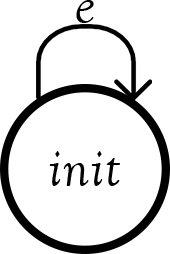
\includegraphics{null}\end{center}
  \item for \(\epsilon\), we have \(M = (\{init\},\ \Sigma^e,\
    \delta,\ init,\ \{init\})\) and graphically, \begin{center}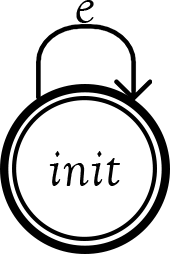
\includegraphics{epsilon}\end{center}
  \item for \(a\), we have \(M = (\{init, accept\},\ \Sigma^e,\
    \delta,\ init,\ \{accept\})\) and graphically, \begin{center}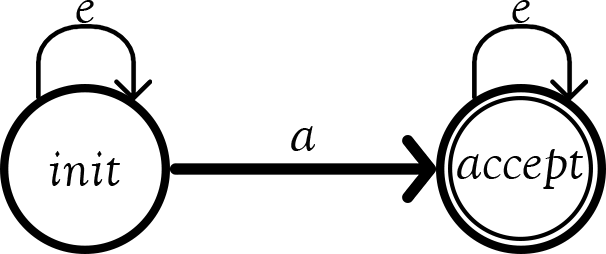
\includegraphics{singleton}\end{center}
  \item suppose \(N_1 = (Q_1,\ \delta_1,\ q_{01},\ F_1)\) and \(N_2 =
    (Q_2,\ \delta_2,\ q_{02},\ F_2)\) are \(\epsilon\)-NFAs translated from the
    regular expressions \(e_1\) and \(e_2\) respectively, then
    \begin{enumerate}[nolistsep]
      \item for \((e_1\ |\ e_2)\), we have \(M = (\{init\} \cup Q_1
        \cup Q_2,\ \Sigma^e,\ \delta,\ init,\ F_1 \cup F_2)\) and
        graphically, \begin{center}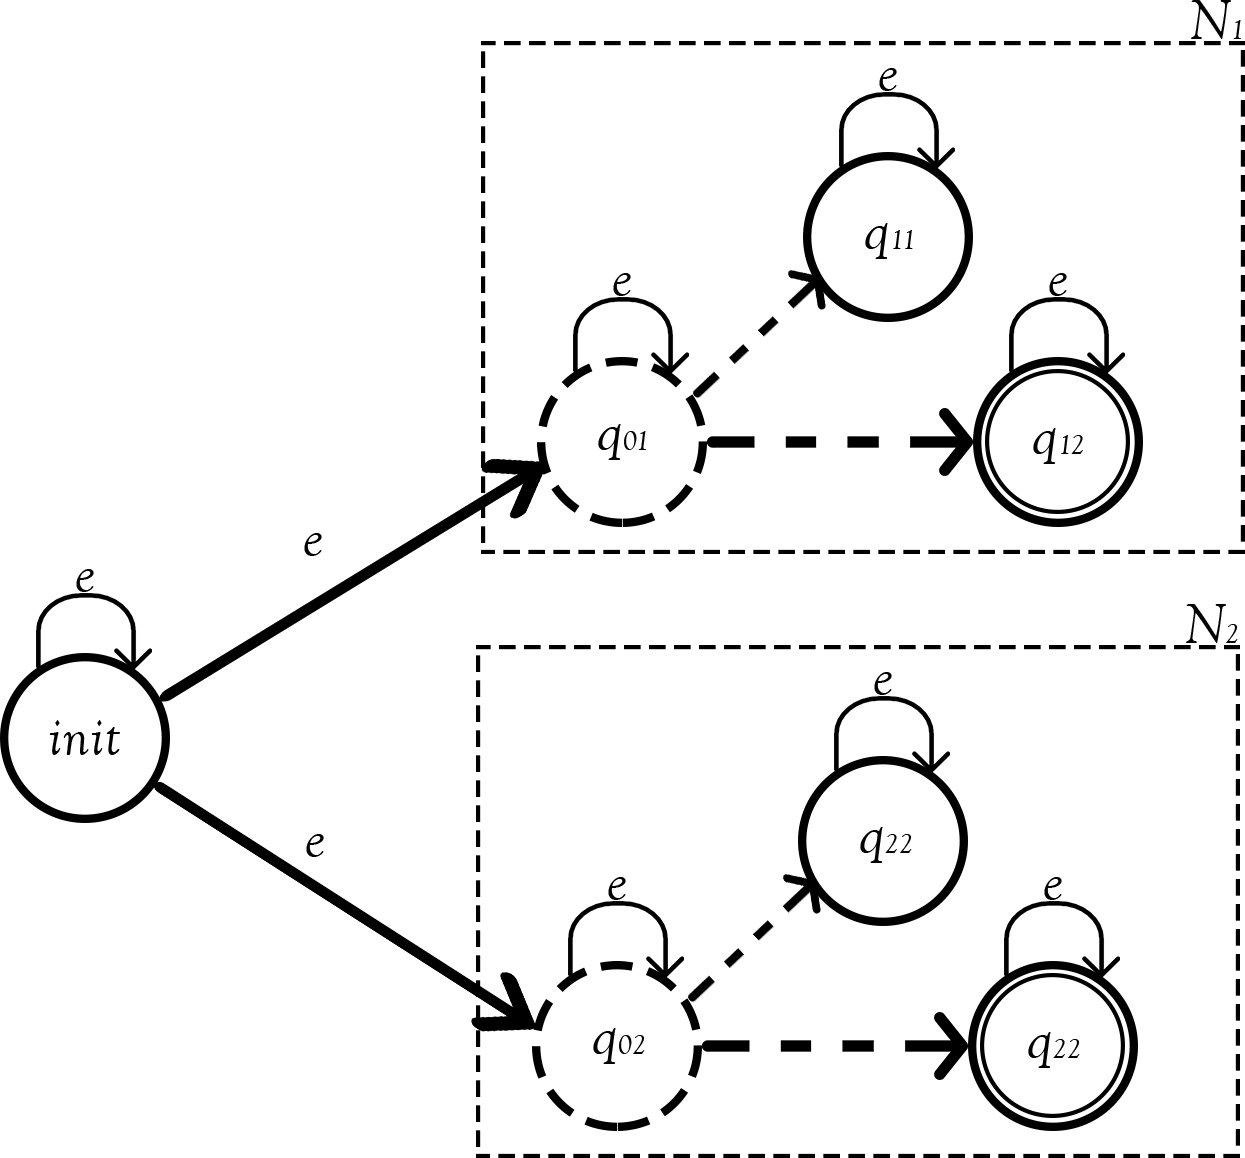
\includegraphics{union}\end{center}
      \item for \(e_1\cdot e_2\), we have \(M = (Q_1 \cup \{mid\}
        \cup Q_2,\ \Sigma^e,\ \delta,\ init,\ F_2)\) and graphically, \begin{center}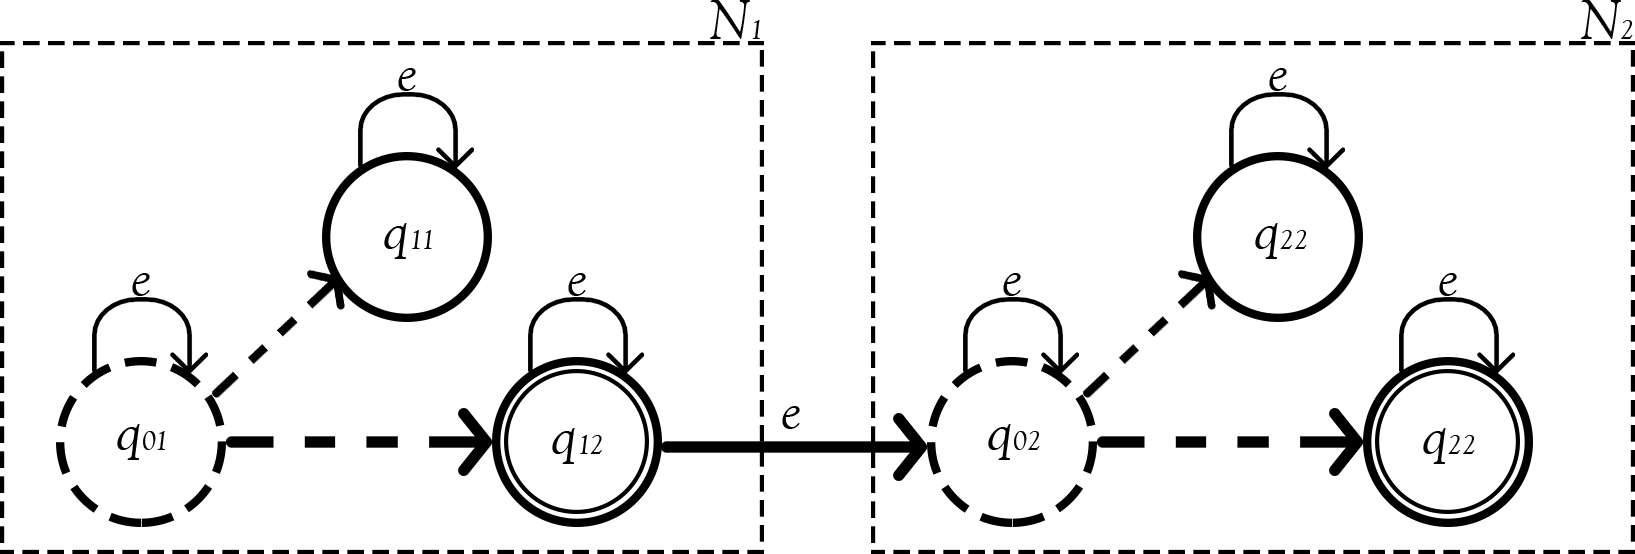
\includegraphics{concat}\end{center}
      \item for \(e_1^{\ *}\), we have \(M = (\{init\} \cup Q_1,\
        \Sigma^e,\ \delta,\ init,\ \{init\} \cup F_1)\) and
        graphically, \begin{center}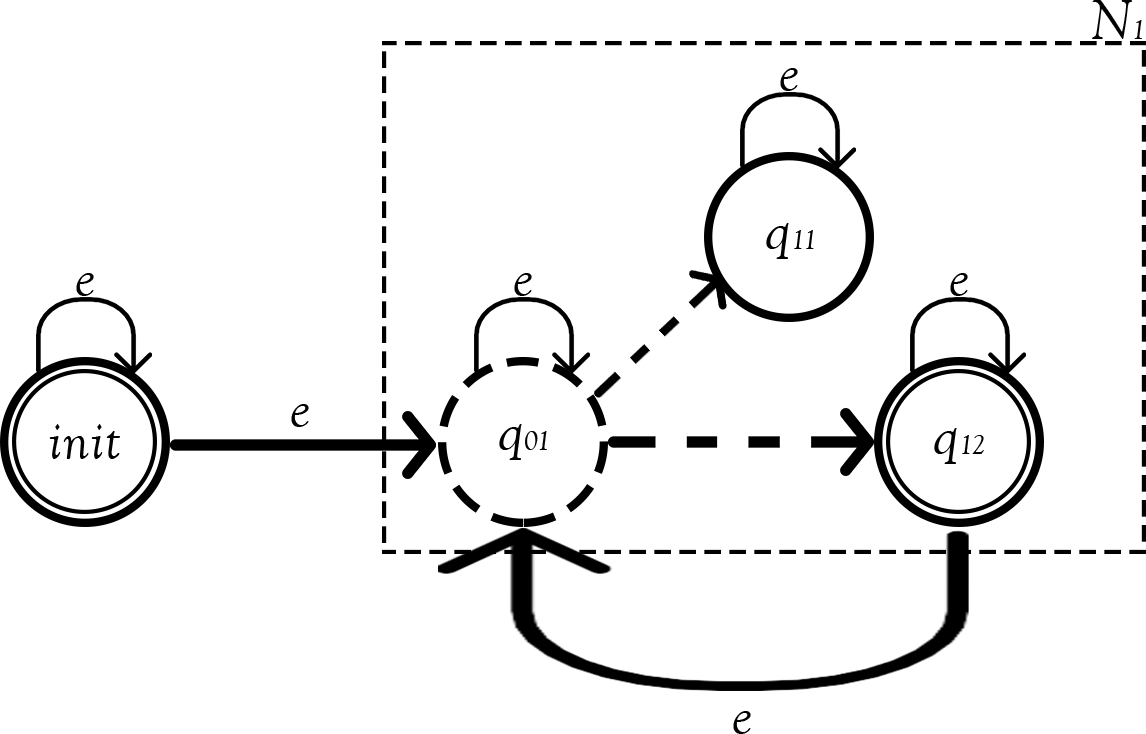
\includegraphics{star}\end{center}
     \end{enumerate}
\end{enumerate}
\end{defn}

\par Apart from the five fields, the other fields in the record
\textit{\(\epsilon\)-NFA} are also constructed by the function. Now, let us prove the correctness of the above translation by
proving that their accepting languages are equal. The correctness
proof is defined as the function \mmb{L^R \!\approx\! L^{eN}} in
\textbf{Correctness.agda} while the detail proofs are
defined in \textbf{Correctness/RegExp-eNFA.agda}. 

\begin{thm} 
\noindent For any given regular expression, \(e\), its accepting
language is equal to the language accepted by the \(\epsilon\)-NFA
translated from \(e\) using Thompson's Construction, i.e. \(L(e) =
L(\)translated \(\epsilon\)-NFA\()\). 
\end{thm} 

\begin{proof}
\noindent We can prove the theorem by induction on regular
expressions. 

\par \noindent \textbf{Base cases.}\quad By \autoref{defn:thompson}, it is
obvious that the statement holds for \(\O\), \(\epsilon\) and
\(a\). 

\par \noindent \textbf{Induction hypothesis 1.}\quad For any two regular expressions
\(e_1\) and \(e_2\), let \(N_1 =
(Q_1,\ \delta_1,\ q_{01},\ F_1)\) and \(N_2 = (Q_2,\ \delta_2,\
q_{02},\ F_2)\) be their translated \(\epsilon\)-NFA 
respectively, we assume that \(L(e_1) = L(N_1)\) and \(L(e_2) =
L(N_2)\). 

\par \noindent \textbf{Inductive steps.}\quad There are three cases: 1)
\(e_1\ |\ e_2\), 2) \(e_1 \cdot e_2\) and 3) \(e_1^{\ *}\). 

\par \noindent 1) \textit{Case \((e_1\ |\ e_2)\)}:\quad Let \(M = (Q,\ \delta,\ q_0,\ F) = (\{init\} \cup Q_1 \cup Q_2,\
\delta,\ init,\ F_1 \cup F_2)\) be its translated \(\epsilon\)-NFA. Then for any string \(w\), 

\par 1.1) if \((e_1\ |\ e_2)\) accepts \(w\), then by
\autoref{defn:regex} and \autoref{defn:lang_union},
either i) \(e_1\) accepts \(w\) or ii) \(e_2\) accepts \(w\). Assuming case i), then by
induction hypothesis, \(N_1\) also accepts \(w\). Therefore, there
must exist an \(\epsilon\)-string of \(w\), \(w^e\), that can take \(q_{01}\)
to an accepting state \(q\) in \(N_1\). Now, consider another
\(\epsilon\)-string of \(w\), \(\epsilon w^e\), it can
take \(init\) to \(q\) in \(M\) because \(\epsilon\) can take \(init\)
to \(q_{01}\). Recall that \(q\) is an accepting
state in \(N_1\); therefore, \(q\) is also an accepting state in
\(M\) and thus, by \autoref{defn:enfa}, \(M\) accepts \(w\). The same argument also applies
to the case when \(e_2\) accepts \(w\); therefore, \(L(e_1\ |\ e_2) \subseteq L(M)\) is true; 

\par 1.2) if \(M\) accepts \(w\), then by \autoref{defn:enfa}, there must exist an
\(\epsilon\)-string of \(w\), \(w^e\), that can take \(init\) to an
accepting state \(q\) in \(M\). \(q\) must be different from \(init\) because
\(q\) is an accepting state but \(init\) is not. Now, by
\autoref{defn:thompson}, there are only two possible ways for \(init\) to reach \(q\) in \(M\), i)
via \(q_{01}\) or ii) via \(q_{02}\). Assuming case i), then \(w^e\)
must be in the form of \(aw'^e\) because \(\epsilon\) is the only alphabet that can take
\(init\) to \(q_{01}\) and thus \(w'^e\) can take \(q_{01}\) to \(q\). Furthermore, \(q\) is an
accepting state in \(M\); therefore, \(q\) is also an accepting
state in \(N_1\) and thus \(N_1\) accepts \(w\). By induction hypothesis, \(e_1\) also accepts \(w\);
therefore, we have \(w \in L(e_1\ |\ e_2)\). The same argument also
applies to case ii) and thus \(L(e_1\ |\ e_2) \supseteq L(M)\) is true; 

\par 1.3) combining 1.1 and 1.2, we have \(L(e_1\ |\ e_2) = L(M)\). 

\par \noindent 2) \textit{Case \((e_1 \cdot e_2)\)}:\quad Let \(M = (Q,\
\delta,\ q_0,\ F) = (Q_1 \cup \{mid\} \cup Q_2,\ \delta,\ q_{01},\
F_2)\) be its translated \(\epsilon\)-NFA. Then for any string
\(w\), 

\par 2.1) if \((e_1 \cdot e_2)\) accepts \(w\), then by
\autoref{defn:regex} and \autoref{defn:lang_con}, there must exist a string \(u \in L(e_1)\) and a string \(v \in L(e_2)\) such that \(w
= uv\). By induction hypothesis, \(N_1\) accepts \(u\) and \(N_2\)
accepts \(v\). Therefore, there must exist i) an \(\epsilon\)-string
of \(u\), \(u^e\), that can take \(q_{01}\) to an accepting state \(q_1\) in
\(N_1\) and ii) an \(\epsilon\)-string of \(v\), \(v^e\), that can take
\(q_{02}\) to an accepting state \(q_2\) in \(N_2\). Now, let us
consider another \(\epsilon\)-string of \(w\), \(u^e\epsilon \epsilon
v^e\), it can take \(q_{01}\) to \(q_2\) in \(M\) because \(u^e\) takes
\(q_{01}\) to \(q_1\), \(\epsilon\) takes \(q_1\) to \(mid\), another
\(\epsilon\) takes \(mid\) to \(q_{02}\) and \(v^e\) takes \(q_{02}\)
to \(q_2\). Furthermore, \(q_2\)
is also an accepting state in \(M\) because \(q_2\) is an accepting
state in \(N_2\). Therefore, \(M\) accepts \(w\)
and thus \(L(e_1 \cdot e_2) \subseteq L(M)\) is true; 

\par 2.2) if \(M\) accepts \(w\), then by \autoref{defn:enfa}, there must
exist an \(\epsilon\)-string of \(w\), \(w^e\), which can take
\(q_{01}\) to an accepting state \(q\) in \(M\). Since \(q\) is an
accepting state in \(M\); therefore, \(q\) must be in \(Q_2\). The only possible way for
\(q_{01}\) to reach \(q\) is by going through the state \(mid\). Therefore, there must exist i) an \(\epsilon\)-string, \(u^e\), that can take
\(q_{01}\) to an accepting state \(q_1\) in \(N_1\) and ii) an
\(\epsilon\)-string \(v^e\) that can take \(q_{02}\) to \(q_2\) in
\(N_1\) and \(w^e = u^e\epsilon\epsilon v^e\). Let \(u\) and \(v\) be the normal strings of \(u^e\) and
\(v^e\) respectively, then we have \(u \in L(N_1)\), \(v \in L(N_2)\) and \(w = uv\). Now, by induction
hypothesis, \(e_1\) accepts \(u\) and \(e_2\) accepts \(v\); and thus
\(e_1 \cdot e_2\) accepts \(w\). Therefore \(L(e_1 \cdot e_2) \supseteq L(M)\) is true; 

\par 2.3) combining 2.1 and 2.2, we have \(L(e_1 \cdot e_2) = L(M)\). 

\par \noindent 3) \textit{Case \(e_1^{\ *}\)}:\quad Let \(M = (Q,\ \delta,\ q_0,\
F) = (Q_1 \cup \{mid\} \cup Q_2,\ \delta,\ q_{01},\ F_2)\) be its
translated \(\epsilon\)-NFA. Then for any string \(w\), 

\par 3.1) if \((e_1^{\ *})\) accepts \(w\), then by \autoref{defn:regex}
and \autoref{defn:lang_star}, there must exist a number \(n\) such
that \(w \in L(e_1)^n\). Now, let us do induction on \(n\). 

\par \quad \textbf{Base case.} \quad When \(n = 0\), then the language
\(L^0\) can only accept the empty string \(\epsilon\); and thus \(w =
\epsilon\). From \autoref{defn:thompson}, it is obvious that \(M\)
accepts \(\epsilon\). 

\par \quad \textbf{Induction hypothesis 2.} \quad Suppose there exists a number \(k\) such that \(w
\in L(e_1)^k\), then \(w\) is also accepted by \(M\). 

\par \quad \textbf{Induction steps.} \quad When \(n = k + 1\), by
\autoref{defn:lang_con} and \autoref{defn:lang_power}, there must
exist a string \(u \in L(e_1)\) and a string \(v \in L(e_1)^k\) such
that \(w=uv\). By induction hypothesis (1), we have \(N_1\) accepts \(u\). Therefore there must exist an \(\epsilon\)-string
\(u\), \(u^e\), that can take \(q_{01}\) to an accepting state \(q\)
in \(N_1\). Since \(q\) is an accepting state; an \(\epsilon\)
alphabet can take \(q\) back to \(q_{01}\). Furthermore, by induction
hypothesis (2), \(M\) also accepts \(v\) which implies that there
exists an \(\epsilon\)-string of \(v\), \(v^e\), that can take
\(init\) to an accepting state \(p\). Since the only
alphabet that can take \(init\) to \(q_{01}\) is \(\epsilon\); therefore,
\(v^e\) must be in the form of \(\epsilon v'^e\). Now, we have proved
that there exists an \(\epsilon\) string of \(w\), \(\epsilon u^e\epsilon v'^e\), that can
take \(init\) to an accepting state \(p\) in \(M\); and thus \(M\)
accepts \(w\). Therefore \(L(e_1^{\ *}) \subseteq L(M)\) is true; 

\par 3.2) if \(M\) accepts \(w\), then by \autoref{defn:enfa}, there must exist an
\(\epsilon\)-string \(w\), \(w^e\), that can take \(init\) to an accepting
state \(q\) with \(n\) transitions in \(M\).  If \(init = q\), then \(w\) must be an empty
string. By \autoref{defn:thompson}, it is obvious that
the empty string is accepted by \(e_1^{\ *}\). If \(init \neq q\),
then there are only two possible ways for \(init\)
to reach \(q\): 1) from \(init\) to \(q\) without going back to
\(q_{01}\) from an accepting state with an \(\epsilon\), we say that this path has no loops and 2) from \(init\)
to \(q\) with at least one loop. 
\par \quad \textit{Case 1}:\quad Since \(q \neq init\), then \(w^e\) must
be in the form of \(\epsilon w'^e\). Recall that the path has no loops, it is
obvious that \(N_1\) accepts \(w\). Therefore by
induction hypothesis (1), \(e_1\) accepts \(w\) and thus \(e_1^{\ *}\)
also accepts \(w\). 
\par \quad \textit{Case 2}:\quad Since \(q \neq init\), then \(w^e\) must
be in the form of \(\epsilon w'^e\). Recall that the path has loops, we
can separate \(w'^e\) into two parts: 1) an \(\epsilon\)-string
\(u^e\) that takes \(init\) to an accepting state \(p\) without loops
and 2) an \(\epsilon\)-string \(\epsilon v^e\) that takes \(p\) to
\(q_{01}\) to \(q\) with loops. Let \(u\) and \(v\) be the normal
string of \(u^e\) and \(\epsilon v^e\) respectively, then it is obvious that
\(w = uv\). By \textit{case 1}, \(e_1\) accepts \(u\). Now, consider
the path from \(q_{01}\) to \(q\). The path must have less than \(n\)
transitions; therefore, we can prove by induction the there must exist a number \(k\) such that
\(L(e_1)^k\) accepts \(v\). Combining the above proofs, we have \(w \in
L(e_1^{\ *})\). 
\par \quad Combining \textit{Case 1} and \textit{Case 2}, we have \(w \in L(e_1^{\ *}) \supseteq L(M)\); 

\par 3.3) combining 3.1 and 3.2, we have \(L(e_1^{\ *}) = L(M)\). 

\par \noindent Therefore, by induction, \(L(e) = L(\)translated
\(\epsilon\)-NFA\()\) is true for all any regular expression \(e\). 
\end{proof}

\par Below is a code snippet of our formalisation of \(L^R \subseteq
L^{eN}\). 

\begin{center} 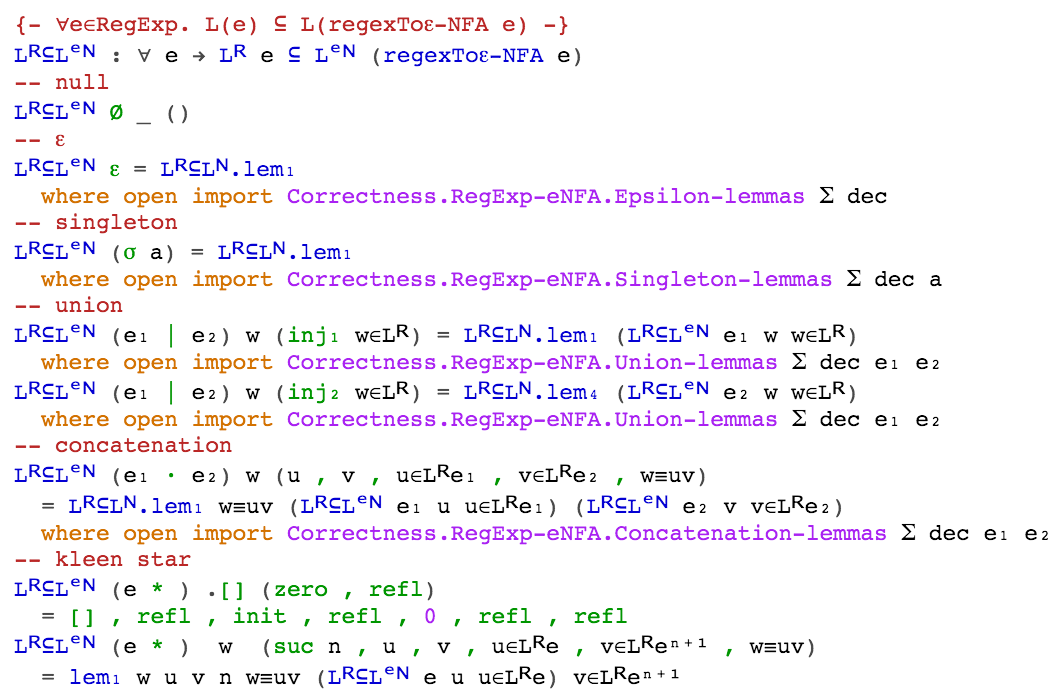
\includegraphics[width=\textwidth]{thm11} \end{center}

\par Pattern matching the regular expression corresponds to the case
analysis in the proof. As shown above, there are six cases:
\(\emptyset\), \(epsilon\), \(\sigma\ a\), union, concatenation and
kleen star. The first three corresponds to the three base
cases. Notice that the recursive calls in last three cases is equivalent to the induction hypothesis of the
proof. These cases are equivalent to the induction steps. 

\subsection{Non-deterministic Finite Automata}
\par Although the definition of NFA is very similar to that of
\(\epsilon\)-NFA, we will still define NFA
separately. The type of NFA is defined in \textbf{NFA.agda} along with
its operations and properties. 

\begin{defn}
\noindent A NFA is a 5-tuple \(M = (Q
,\ \Sigma,\ \delta,\ q_0,\ F)\), where
\begin{enumerate}[nolistsep]
  \item \(Q\) is a finite set of states;
  \item \(\Sigma\) is the set of alphabets;
  \item \(\delta\) is a mapping from \(Q \times \Sigma\) to
    \(\mathcal P \left({Q}\right)\) that defines the behaviour of the automata;
  \item \(q_0\) in \(Q\) is the initial state;
  \item \(F \subseteq Q\) is the set of accepting states. 
\end{enumerate}
\end{defn}

\par It is formalised as a record in Agda as shown below: 

\begin{lstlisting}[mathescape=true,xleftmargin=.3\textwidth]
record NFA : Set$_1$ where
  field
    Q      : Set
    $\delta$       : Q $\to$ $\Sigma$ $\to$ DecSubset Q
    q$_0$      : Q
    F      : DecSubset Q
    Q?     : DecEq Q
    |Q|-1  : $\mathbb{N}$
    It     : Vec Q (suc |Q|-1)
    $\forall$q$\in$It    : (q : Q) $\to$ (q $\in^V$ It)
    unique : Unique It
\end{lstlisting}

\par The set of alphabets \(\Sigma\) is passed into the module as a
parameter. Together with \(Q\), \(\delta\),
\(q_0\) and \(F\), these five fields correspond to the 5-tuple
NFA. The other extra fields are used in powerset construction. They
are \(Q?\) -- the decidable equality of \(Q\);
\(|Q|-1\) -- the number of states minus 1; \(It\) -- a vector containing every state in \(Q\); \(\forall q\in It\)
-- a proof that every state in \(Q\) is also in the vector
\(It\); and \(unique\) -- a proof that there is no repeating elements in
\(It\). 

\par Now, before we can define the accepting language of a given
NFA, we need to define several operations of NFA. 

\begin{defn}
\noindent A configuration is composed of a state and an alphabet from
\(\Sigma\), i.e. \(C = Q \times \Sigma\). 
\end{defn}

\begin{defn}
\noindent A move in an NFA is
represented by a binary function (\(\vdash\)) on two configurations. We say
that for all \(w \in \Sigma^*\) and \(a \in \Sigma\), \((q, aw)
\vdash (q' , w)\) if and only if \(q' \in \delta (q , a)\). 
\end{defn}

\par The binary function is defined in Agda as follow: 
\begin{lstlisting}[mathescape=true,xleftmargin=.3\textwidth]
  _$\vdash$_ : (Q $\times$ $\Sigma$ $\times$ $\Sigma^*$) $\to$ (Q $\times$ $\Sigma^*$) $\to$ Set
  (q , a , w) $\vdash$ (q' , w') = w $\equiv$ w' $\times$ q' $\in^d$ $\delta$ q a
\end{lstlisting}

\begin{defn}
\noindent Suppose \(C\) and \(C'\) are configurations. We say that \(C \vdash^0 C'\) if and only
if \(C = C'\); and \(C_0 \vdash^k C_k\) for any \(k \geq 1\) if and only if there exists a chain of
configurations \(C_1, C_2, ..., C_{k-1}\) such that \(C_i \vdash C_{i+1}\) for all \(0 \leq i < k\). 
\end{defn}

\par It is defined as a recursive function in Agda as follow: 
\begin{lstlisting}[mathescape=true,xleftmargin=.3\textwidth]
  _$\vdash^k$_-_ : (Q $\times$ $\Sigma^*$) $\to$ $\mathbb{N}$ $\to$ (Q $\times$ $\Sigma^*$) $\to$ Set
  (q , w) $\vdash^k$ zero  - (q' , w')
    = q $\equiv$ q' $\times$ w $\equiv$ w'
  (q , w) $\vdash^k$ suc n - (q' , w') 
    = $\exists$[ p $\in$ Q ] $\exists$[ a $\in$ $\Sigma$ ] $\exists$[ u $\in$ $\Sigma^*$ ]
      (w $\equiv$ a :: u $\times$ (q , a , u) $\vdash$ (p , u) $\times$ (p , u) $\vdash^k$ n - (q' , w'))
\end{lstlisting}

\begin{defn}
\noindent We say that \(C \vdash^* C'\) if and only
if there exists a number of chains \(n\) such that \(C \vdash^n C'\). 
\end{defn}

\par Its corresponding type is defined as follow: 
\begin{lstlisting}[mathescape=true,xleftmargin=.3\textwidth]
  _$\vdash^*$_ : (Q $\times$ $\Sigma^*$) $\to$ (Q $\times$ $\Sigma^*$) $\to$ Set
  (q , w) $\vdash^*$ (q' , w') = $\exists$[ n $\in$ $\mathbb{N}$ ] (q,w) $\vdash^k$ n - (q',w')
\end{lstlisting}

\begin{defn}
\noindent For any string \(w\), it is accepted by an NFA
if and only \(w\) can take \(q_0\) to an accepting state \(q\). Therefore, the
accepting language of an NFA is given by the set \(\{w\ |\ \exists q\in F.\ (q_0,w) \vdash^* (q,\epsilon)\}\). 
\end{defn}

\par The corresponding formalisation in Agda is as follow: 
\begin{lstlisting}[mathescape=true,xleftmargin=.3\textwidth]
  L$^N$ : NFA $\to$ Language
  L$^N$ nfa = $\lambda$ w $\to$ 
            $\exists$[ q $\in$ Q ] (q $\in^d$ F $\times$ (q$_0$ , w) $\vdash^*$ (q , [])))
\end{lstlisting} 


\subsection{Removing \(\epsilon\)-transitions}
\par The translation of \(\epsilon\)-NFA to NFA is defined in
\textbf{Translation/eNFA-NFA.agda}. In order to remove all the \(\epsilon\)-transitions, we need to
know whether a state \(q\) can reach another state \(q'\) with only
\(\epsilon\)-transitions. Let us begin by defining such a relation on states. 

\begin{defn}
\noindent We say that
\(q \to_\epsilon^0 q'\) if and only if
\(q\) is equal to \(q'\); and \(q \to_\epsilon^k q'\) for \(k \geq
1\) if and only if \(q\) can be transited to \(q'\) with \(k\)
\(\epsilon\)-transitions. We call this an \(\epsilon\)-path from \(q\) to \(q'\).
\end{defn}

\par It is defined as a recursive function in Agda as follow:
\begin{lstlisting}[mathescape=true,xleftmargin=.3\textwidth]
_$\to_\epsilon^k$_-_ : Q $\to$ $\mathbb{N}$ $\to$ Q $\to$ Set
q $\to_\epsilon^k$ zero - q' = q $\equiv$ q'
q $\to_\epsilon^k$ suc n - q' = $\exists$[ p $\in$ Q ] ( p $\in^d$ $\delta$ q E $\times$ p $\to_\epsilon^k$ n - q' )
\end{lstlisting}

\begin{defn}
\noindent We say that \(q \to_\epsilon^* q'\) if and only if there
exists an \(\epsilon\)-path from \(q\) to \(q'\) with \(n\) transitions, i.e. \(\exists n.\ q \to_\epsilon^n q'\). 
\end{defn}

\par The corresponding type is as follow: 
\begin{lstlisting}[mathescape=true,xleftmargin=.3\textwidth]
_$\to_\epsilon^*$_ : Q $\to$ Q $\to$ Set
q $\to_\epsilon^*$ q' = $\exists$[ n $\in$ $\mathbb{N}$ ] q $\to_\epsilon^k$ n - q'
\end{lstlisting}

\par Now we have to prove that for any two states \(q\) and \(q'\), 
\(q \to_\epsilon^* q'\) is decidable. However, it is not possible to
prove it directly because the set of natural numbers is
infinite. Therefore, we will introduce an algorithm that computes the
\(\epsilon\)-closure of a state. The \(\epsilon\)-closure of a state
\(q\), \(\epsilon\hyphen closure(q)\) should contain all the states
that are reachable from \(q\) with only \(\epsilon\)-transitions. We will prove that for any two states
\(q\) and \(q'\), \(q \to_\epsilon^* q'\) if and only if \(q' \in \epsilon\hyphen closure(q)\). By proving that they are equivalent, we
will have proved the decidability of \(q \to_\epsilon^* q'\). 

\begin{defn}
\noindent For any given state \(q\), \(\epsilon\hyphen closure(q)\) is obtained by: 
\begin{enumerate}[nolistsep]
  \item put \(q\) into a subset \(S\), i.e. \(S = \{q\}\)
  \item loop for \(|Q| - 1\) times: 
  \begin{enumerate}
    \item for every state \(p\) in \(S\), if \(\epsilon\) can take
      \(p\) to another state \(r\), i.e. \(r \in
        \delta (p,\epsilon)\), then put \(r\) into \(S\). 
  \end{enumerate}
  \item the result subset \(S\) is the \(\epsilon\)-closure of \(q\)
\end{enumerate}
\end{defn}

\begin{lem}
\noindent For any two states \(q\) and \(q'\), \(q \to_\epsilon^* q'\)
if and only if \(q' \in \epsilon\hyphen closure(q)\). 
\end{lem}

\begin{proof}
\noindent We have to prove for both directions. 
\par \noindent 1) If \(q \to_\epsilon^* q'\), then there must exist a
number \(n\) such that \(\epsilon^n\) can take \(q\) to \(q'\). If
\(n < |Q|\), then it is obvious that \(q' \in
\epsilon\hyphen closure(q)\) is true. If \(n \geq |Q|\), the
\(\epsilon\)-path from \(q\) to \(q'\) must have loop(s) inside. By
removing the loop(s), the equivalent \(\epsilon\)-path must have at
most \(|Q|-1\) \(\epsilon\)-transitions. Therefore, \(q' \in
\epsilon\hyphen closure(q)\) is true. 

\par \noindent 2) If \(q' \in \epsilon\hyphen closure(q)\), it is obvious
that \(q \to_\epsilon^{|Q|-1} q'\) must be true and thus \(q
\to_\epsilon^* q'\) is true. 
\end{proof}

\par Since we have proved that they are equivalent; therefore the
decidability of \(q \to_\epsilon^* q'\) follows. Now, let us define
the translation of \(\epsilon\)-NFA to NFA using \(q \to_\epsilon^* q'\). 
 
\begin{defn}
\label{defn:remove_epsilon}
\noindent For a given \(\epsilon\)-NFA, \((Q,\ \delta,\
q_0,\ F)\), its translated NFA will be \((Q,\ \delta',\ q_0,
F')\) where
\begin{itemize}[nolistsep]
  \item \(\delta'(q,a) = \delta (q,a) \cup \{q'\ |\ \exists p.\
      q \to_\epsilon^* p \wedge q' \in \delta (p,a)\}\);
  \item \(F' = F \cup \{q\ |\ \exists p\in F.\ q \to_\epsilon^* p\}
    \). 
\end{itemize}
\end{defn}

\par Now, let us prove the correctness of the above translation by proving their accepting languages
are equal. The correctness proofs can be found in \textbf{Correctness/eNFA-NFA.agda}.

\begin{thm}
\noindent For any \(\epsilon\)-NFA, its accepting language is equal to
the language accepted by its translated NFA, i.e. \(L(\epsilon\)-NFA\()
= L(\)translated NFA\()\). 
\end{thm}

\begin{proof}
\noindent Let the \(\epsilon\)-NFA be \(\epsilon N = (Q,\ \delta,\ q_0,\
F)\), and its translated NFA be \(N = (Q,\ \delta',\ q_0,\ F')\)
according to \autoref{defn:remove_epsilon}. To
prove the theorem, we have to prove that \(L(\epsilon N) \subseteq
L(N)\) and \(L(\epsilon N) \supseteq L(N)\). Then for any string \(w\), 

\par \noindent 1) if \(\epsilon N\) accepts \(w\), then there must exist an
\(\epsilon\)-string of \(w\), \(w^e\), that can take \(q_0\) to an
accepting state \(q\) with \(n\) transitions. There are three
possibilities: a) the last transition in the path is not an
\(\epsilon\)-transition, b) the path is divided into three parts, the
first part from \(q_0\) to a state \(p\) with less than \(n\)
transitions; the second part from \(p\) to a state \(p_1\) with an
alphabet \(a\) and the third part from \(p_1\) to \(q\) with only
\(\epsilon\)-transitions and c) the path from \(q_0\)
to \(q\) consists of only \(\epsilon\)-transitions.

\par \textit{Case a}:\quad There must exist a state \(p\), an
\(\epsilon\)-string \(u^e\), and an alphabet \(a\) such that \(u^e\)
can take \(q_0\) to \(p\) in less than \(n\) transitions, \(q \in
\delta(p,a)\) and \(w^e = u^ea\). Since that path from \(q_0\) to
\(p\) is less than \(n\) transitions; therefore, we can prove by
induction that the normal string of \(u^e\), \(u\), can take
\(q_0\) to \(p\) in \(N\). Furthermore, \(w = ua\); therefore, \(w\) can
take \(q_0\) to \(q\) in \(N\) and thus \(N\) accepts \(w\). 

\par \textit{Case b}:\quad There must exist two states \(p\) and \(p_1\), an
\(\epsilon\)-string of \(w\), \(u^e\), and an alphabet \(a\) such
that \(u^e\) can take \(q_0\) to \(p\) in less than \(n\) transitions,
\(p_1 \in \delta(p,a)\), \(p_1 \to_\epsilon^* q\) and \(w = ua\). Since that path from \(q_0\) to
\(p\) is less than \(n\) transitions; therefore, we can prove by
induction that the normal string of \(u^e\), \(u\), can take
\(q_0\) to \(p\) in \(N\). Furthermore, \(p_1\) must be an accepting state in \(N\)
because it can be transited to an accepting state \(q\) with only
\(\epsilon\)-transitions. Therefore, \(w\) can take \(q_0\) to an
accepting state \(p_1\) in \(N\) and thus \(N\) accepts \(w\). 

\par \textit{Case c}:\quad If the path from \(q_0\)
to \(q\) consists of only \(\epsilon\)-transitions, then \(q_0
\to_\epsilon^* q\) is true; therefore, \(q_0\) is also an accepting
state in \(N\). Furthermore, the accepted string consists of \(\epsilon\) only;
therefore, \(w = \epsilon\). It is obvious that \(N\) accepts \(\epsilon\). 

\par \noindent 2) if \(N\) accepts \(w\), then \(w\) must be able to take \(q_0\) to an
accepting state \(q\). Since \(q\) is an accepting state, then \(q\)
is also an accepting state in \(\epsilon N\) or there exists a state 
\(p\) such that \(q \to_\epsilon^* p\) and \(p \in F\). For the former
case, since \(w\) is also an \(\epsilon\)-string of itself; therefore,
it is obvious that \(\epsilon N\) accepts \(w\). For the latter
case, suppose the path from \(q\) to \(p\) has \(n\)
\(\epsilon\)-transitions, the consider another \(\epsilon\)-string of
\(w\), \(w\epsilon^n\), it can take \(q_0\) to \(p\) in
\(\epsilon N\). Therefore \(\epsilon N\) accepts \(w\). 
\end{proof}

\section{Deterministic Finite Automata}
\par The type of DFA is defined in \textbf{DFA.agda} along with its
operations and properties. 

\begin{defn}
\noindent A DFA is a 5-tuple \(M = (Q
,\ \Sigma,\ \delta,\ q_0,\ F)\), where
\begin{enumerate}[nolistsep]
  \item \(Q\) is a finite set of states;
  \item \(\Sigma\) is the set of alphabets;
  \item \(\delta\) is a mapping from \(Q \times \Sigma\) to \(Q\) that defines the behaviour of the automata;
  \item \(q_0\) in \(Q\) is the initial state;
  \item \(F \subseteq Q\) is the set of accepting states. 
\end{enumerate}
\end{defn}

\par It is formalised as a record in Agda as shown below: 

\begin{lstlisting}[mathescape=true,xleftmargin=.3\textwidth]
record DFA : Set$_1$ where
  field
    Q      : Set
    $\delta$       : Q $\to$ $\Sigma$ $\to$ DecSubset Q
    q$_0$      : Q
    F      : DecSubset Q
    _$\approx$_     : Q $\to$ Q $\to$ Set
    $\approx\hyphen$isEquiv : IsEquivalence _$\approx$_
    $\delta\hyphen$lem    : $\forall$ {q} {p} a $\to$ q $\approx$ p $\to$ $\delta$ q a $\approx$ $\delta$ p a
    F$\hyphen$lem   : $\forall$ {q} {p}   $\to$ q $\approx$ p $\to$ q $\in^d$ F $\to$ p $\in^d$ F
\end{lstlisting}

\par The set of alphabets \(\Sigma\) is passed into the module as a
parameter. Together with \(Q\), \(\delta\),
\(q_0\) and \(F\), these five fields correspond to the 5-tuple
DFA. The other extra fields are used in proving its decidability. They
are \(\_\approx\_\) -- an equivalence relation on states;
\(\approx\hyphen isEquiv\) -- a proof that the relation \(\approx\) is
an equivalence relation; \(\delta\hyphen lem\) -- a proof that for any
alphabet \(a\) and any two states \(q\) and \(p\), if \(q \approx p\)
then \(\delta (q,a) \approx \delta (p,a)\); and \(F\hyphen lem\) -- a
proof that for any two states \(q\) and \(p\), if \(q \approx p\) and
\(q\) is an accepting state, then \(p\) is also an accepting state. 

\par Now, before we can define the accepting language of a given
DFA, we need to define several operations of DFA. 

\begin{defn}
\noindent A configuration is composed of a state and an alphabet from
\(\Sigma\), i.e. \(C = Q \times \Sigma\). 
\end{defn}

\begin{defn}
\noindent A move in an DFA is
represented by a binary function (\(\vdash\)) on two configurations. We say
that for all \(w \in \Sigma^*\) and \(a \in \Sigma\), \((q, aw)
\vdash (q' , w)\) if and only if \(q' = \delta (q , a)\). 
\end{defn}

\par The binary function is defined in Agda as follow: 
\begin{lstlisting}[mathescape=true,xleftmargin=.3\textwidth]
  _$\vdash$_ : (Q $\times$ $\Sigma$ $\times$ $\Sigma^*$) $\to$ (Q $\times$ $\Sigma^*$) $\to$ Set
  (q , a , w) $\vdash$ (q' , w') = w $\equiv$ w' $\times$ q' $\approx$ $\delta$ q a
\end{lstlisting}

\begin{defn}
\noindent Suppose \(C\) and \(C'\) are configurations. We say that \(C \vdash^0 C'\) if and only
if \(C = C'\); and \(C_0 \vdash^k C_k\) for any \(k \geq 1\) if and only if there exists a chain of
configurations \(C_1, C_2, ..., C_{k-1}\) such that \(C_i \vdash C_{i+1}\) for all \(0 \leq i < k\). 
\end{defn}

\par It is defined as a recursive function in Agda as follow: 
\begin{lstlisting}[mathescape=true,xleftmargin=.3\textwidth]
  _$\vdash^k$_-_ : (Q $\times$ $\Sigma^*$) $\to$ $\mathbb{N}$ $\to$ (Q $\times$ $\Sigma^*$) $\to$ Set
  (q , w) $\vdash^k$ zero  - (q' , w')
    = q $\equiv$ q' $\times$ w $\equiv$ w'
  (q , w) $\vdash^k$ suc n - (q' , w') 
    = $\exists$[ p $\in$ Q ] $\exists$[ a $\in$ $\Sigma$ ] $\exists$[ u $\in$ $\Sigma^*$ ]
      (w $\equiv$ a :: u $\times$ (q , a , u) $\vdash$ (p , u) $\times$ (p , u) $\vdash^k$ n - (q' , w'))
\end{lstlisting}

\begin{defn}
\noindent We say that \(C \vdash^* C'\) if and only
if there exists a number of chains \(n\) such that \(C \vdash^n C'\). 
\end{defn}

\par Its corresponding type is defined as follow: 
\begin{lstlisting}[mathescape=true,xleftmargin=.3\textwidth]
  _$\vdash^*$_ : (Q $\times$ $\Sigma^*$) $\to$ (Q $\times$ $\Sigma^*$) $\to$ Set
  (q , w) $\vdash^*$ (q' , w') = $\exists$[ n $\in$ $\mathbb{N}$ ] (q,w) $\vdash^k$ n - (q',w')
\end{lstlisting}

\begin{defn}
\noindent For any string \(w\), it is accepted by an DFA
if and only \(w\) can take \(q_0\) to an accepting state \(q\). Therefore, the
accepting language of an DFA is given by the set \(\{w\ |\ \exists q\in F.\ (q_0,w) \vdash^* (q,\epsilon)\}\). 
\end{defn}

\par The corresponding formalisation in Agda is as follow: 
\begin{lstlisting}[mathescape=true,xleftmargin=.3\textwidth]
  L$^D$ : DFA $\to$ Language
  L$^D$ dfa = $\lambda$ w $\to$ 
            $\exists$[ q $\in$ Q ] (q $\in^d$ F $\times$ (q$_0$ , w) $\vdash^*$ (q , [])))
\end{lstlisting} 


\section{Powerset Construction}
\par The translation of NFA to DFA is defined as the function
\textbf{powerset-construction} in \textbf{Translation/NFA-DFA.agda}. 

\begin{defn}
\label{defn:powerset}
\noindent For any given NFA, \((Q,\ \delta,\ q_0,\ F)\), its
translated DFA will be \((\mathcal P \left({Q}\right),\ \delta',\ \{q_0\},\ F')\) where
\begin{itemize}[nolistsep]
  \item \(\delta'(qs,a) = \{q'\ |\ \exists q\in qs.\ q' \in \delta (q,a)\}\);
  \item \(F' = \{qs\ |\ \exists q\in F.\ q \in qs\}\). 
\end{itemize}
\end{defn}

\par In Agda, the set \(\mathcal P \left({Q}\right)\) is defined as
the set of decidable subsets, i.e. \(Q' = DecSubset Q\). Therefore,
the decidability of the set \(\delta'(qs,a)\) and \(F'\) must be
proved using the vector represenation of \(Q\). The corresponding
proofs are defined in the module \textbf{Powerset-Construction} in the
same file. 

\par Now, before proving that their accepting languages are equal, we 
need to prove the following lemmas which can be found in
\textbf{Correctness/NFA-DFA.agda}. 

\begin{lem}
\label{lem:nfa<dfa}
\noindent Let a NFA be \(N = (Q,\ \delta,\ q_0,\ F)\) and its
translated DFA be \(D = (\mathcal P \left({Q}\right),\ \delta',\ {q_0},
F')\) according to \autoref{defn:powerset}. For any string \(w\), if \(w\) can take \(q_0\) to a state
\(q\) with \(n\) transitions in \(N\), then there must exist a subset \(qs\) such that \(q
\in qs\) and \(w\) can take \(\{q_0\}\) to \(qs\) in \(D\),
i.e. \(\forall w.\exists q.\exists n.\ (q_0,w) \vdash^n (q,w) \Rightarrow
\exists qs.\ q \in qs \wedge ({q_0},w) \vdash^* (qs,\epsilon)\). 
\end{lem}

\par The proof is defined as the function \mmb{lem_1} under the module
\mmb{L^N\!\subseteq L^D}. 

\begin{proof}
\noindent We can prove the lemma by induction on \(n\).
\par \noindent \textbf{Base case.}\quad If \(n = 0\), then \(q_0 = q\)
and \(w = \epsilon\). It is obvious that the statement holds.

\par \noindent \textbf{Induction hypothesis.}\quad For any string \(w\), if \(w\) can take \(q_0\) to a state
\(q\) with \(k\) transitions in \(N\), then there exists a subset \(qs\) such that \(q
\in qs\) and \(w\) can take \(\{q_0\}\) to \(qs\) in \(D\). 

\par \noindent \textbf{Induction step.}\quad If \(n = k + 1\), then
\(w\) can take \(q_0\) to a state \(q\) by \(k + 1\) transitions. Let
\(w = w'a\) where \(a\) is an alphabet, then \(w'\) can take \(q_0\)
to a state \(p\) by \(k\) transitions and \(q \in \delta(p,a)\). By induction hypothesis, there must exist a subset \(ps\) such that \(p
\in ps\) and \(w'\) can take \(\{q_0\}\) to \(ps\) in \(D\). Furthermore, since \(q \in \delta(p,a)\), then \(a\) must be
able to take \(ps\) to a subset \(qs\) where \(q \in qs\). Therefore,
there exists a subset \(qs\) such that \(q \in qs\) and \(w\) can take
\(\{q_0\}\) to \(qs\); and thus the statement is true. 
\end{proof}

\begin{lem}
\label{lem:nfa>dfa}
\noindent Let a NFA be \(N = (Q,\ \delta,\ q_0,\ F)\) and its
translated DFA be \(D = (\mathcal P \left({Q}\right),\ \delta',\ {q_0},
F')\) according to \autoref{defn:powerset}. For any string \(w\), any
number \(n\) and any two states \(qs\) and \(ps\) in \(\mathcal P \left({Q}\right)\), if
\((qs,w) \vdash^n (ps,\epsilon)\) then \(ps =
\{p\ |\ \exists q\in qs.\ (q,w) \vdash^n (p,\epsilon)\}\). 
\end{lem}

\par The proof is defined as the function \mmb{lem_2} under the module
\mmb{L^N\!\supseteq L^D}. 

\begin{proof}
\noindent We can prove the lemma by induction on \(n\). 

\par \noindent \textbf{Base case.}\quad If \(n = 0\), then \(qs = ps\)
and \(w = \epsilon\). Then for any state \(p\) in \(Q\), 
\par \noindent  1) if \(p \in ps\), then \(p\) is also in \(qs\). It is obvious that
\((p,\epsilon) \vdash^0 (p, \epsilon)\) is true; therefore, \(p \in
\{p\ |\ \exists q\in qs.\ (q,w) \vdash^0 (p,\epsilon)\}\); 
\par \noindent  2) if \(p \in \{p\ |\ \exists q\in qs.\ (q,w) \vdash^0
(p,\epsilon)\}\), then \(p\) must be in \(qs\) and thus \(p \in ps\). 

\par \noindent \textbf{Induction hypothesis.}\quad For any string \(w\) and any
two states \(qs\) and \(ps\) in \(\mathcal P \left({Q}\right)\), if
\((qs,w) \vdash^k (ps,\epsilon)\) then \(ps =
\{p\ |\ \exists q\in qs.\ (q,w) \vdash^k (p,\epsilon)\}\). 

\par \noindent \textbf{Induction step.}\quad If \(n = k + 1\), then
\(w\) must be able to take \(qs\) to \(ps\) with \(k + 1\)
transitions in \(D\). Therefore there must exist an alphabet \(a\)
that can take \(qs\) to a subset \(rs\),
i.e. \(rs = \delta'(qs,a)\); and a string \(u\) that can take \(rs\) to
\(ps\) with \(k\) transitions. By induction hypothesis, we have \(ps =
\{p\ |\ \exists r\in rs.\ (r,u) \vdash^k (p,\epsilon)\}\). Then for any state \(p\) in \(Q\), 

\par \noindent  1) if \(p \in ps\), then there must exist a state \(r \in rs\)
such that \((r,u) \vdash^k (p,\epsilon)\). Since \(rs =
\delta'(qs,a)\); therefore, \(r \in \delta'(qs,a)\) and thus there
exists a state \(q \in qs\) such that \(r \in \delta (q,a)\). Therefore,
\((q,w) \vdash^{k+1} (p,\epsilon)\) is true and thus \(p \in \{p\ |\ \exists q\in qs.\ (q,w) \vdash^{k+1}
(p,\epsilon)\}\). 

\par \noindent  2) if \(p \in \{p\ |\ \exists q\in qs.\ (q,w) \vdash^{k+1}
(p,\epsilon)\}\), then there exists a state \(q \in qs\) such that \((q,w) \vdash^{k+1}
(p,\epsilon)\). Also, there must exist a state \(r \in Q\) such that
\(r \in \delta (q,a)\) and the string \(u\) can take \(r\) to \(p\) in
\(N\). Since, \(q
\in qs\) and \(r \in \delta (q,a)\); therefore, \(r \in \delta'(qs,a)
= rs\) and thus \(p \in \{p\ |\ \exists r\in rs.\ (r,u) \vdash^k
(p,\epsilon)\} = ps\). 
\end{proof}

\par Now, by using the above lemmas, we can prove the correctness of
the translation by proving that their accepting languages are
equal. The correctness proof is defined as the function \mmb{L^N
  \!\approx\! L^D} in \textbf{Correctness.agda} while the detail
proofs are defined in \textbf{Correctness/NFA-DFA.agda}. 

\begin{thm}
\noindent For any NFA, its accepting language is equal to
the language accepted by its translated DFA, i.e. \(L(\)NFA\()
= L(\)translated DFA\()\). 
\end{thm}

\begin{proof}
\noindent For a given NFA, \(N = (Q,\ \delta,\ q_0,\ F)\), let its
translated DFA be \(D = (\mathcal P \left({Q}\right),\ \delta',\
{q_0},\ F')\). To
prove the theorem, we have to prove that \(L(N) \subseteq L(D)\) and
\(L(N) \supseteq L(D)\). For any string \(w\), 

\par \noindent 1) if \(N\) accepts \(w\), then \(w\) can take \(q_0\) to an
accepting state \(q\) with \(n\) transitions in \(N\). By
\autoref{lem:nfa<dfa}, there must exist a subset \(qs\) such that
\(q \in qs\) and \(w\)
can take \(\{q_0\}\) to \(qs\) in \(D\). Since \(q\) is
an accepting state; therefore, \(qs\) is also an accepting state in
\(D\) and thus \(D\) accepts \(w\). 

\par \noindent 2) if \(D\) accepts \(w\), then \(w\) can take
\(\{q_0\}\) to an accepting state \(qs\) in \(D\) with \(n\)
transitions. Since \(qs\) is an accepting state, therefore, there must
exist a state \(q\) in \(Q\) such that \(q \in qs\) and \(q\) is also
an accepting state in \(N\). Assuming \(w\) cannot take \(q_0\) to
\(q\) in \(N\) for any number of transitions, then by
\autoref{lem:nfa>dfa}, \(qs = \emptyset\) and thus \(q \notin qs\) which contradicts the assumption that \(q \in
qs\). Therefore, \(w\) must be able to take \(q_0\) to \(q\) in \(N\) and thus \(N\) accepts \(w\). 
\end{proof}


\section{Decidability of DFA and Regular Expressions}
\par Recall that the accepting language of a DFA is given by the set
\(\{w\ |\ \exists q\in F.\ (q_0,w) \vdash^* (q,\epsilon)\}\), which is
equivalent to the set \(\{w\ |\ \exists q\in F.\ \exists n.\ (q_0,w) \vdash^n (q,\epsilon)\}\). 
Its decidability cannot be proved directly because the set of natural
numbers is infinite. Therefore, we have to
introduce another representation and prove
that they are equivalent. The representation and the related lemmas are
defined under the module \textbf{DFA-Operations} in \textbf{DFA.agda}. 

\begin{defn}
\noindent We define a function \(\delta^*(q,w)\) that takes a state \(q\) and
a string \(w\) as the arguments and returns a state \(p\) after
running the DFA. It is defined recursively as follow: 
\begin{lstlisting}[mathescape=true,xleftmargin=.3\textwidth]
$\delta^*$ : Q $\to$ $\Sigma^*$ $\to$ Q
$\delta^*$ q [] = q
$\delta^*$ (a :: w) = $\delta^*$ ($\delta$ q a) w
\end{lstlisting}
\end{defn}

\begin{defn}
\noindent We define \(\delta_0(w)\) as the function that runs the DFA
from \(q_0\) with a string \(w\). 
\begin{lstlisting}[mathescape=true,xleftmargin=.3\textwidth]
$\delta_0$ : $\Sigma^*$ $\to$ Q
$\delta_0$ w = $\delta^*$ $q_0$ w
\end{lstlisting}
\end{defn}

\par Now, before proving that the two representations are equivalent, we have to prove the following lemmas. 

\begin{lem}
\label{lem:dec_iff}
\noindent For any state \(q\) and any string \(w\), \(\delta^*(q,w) \in F\) if and only
if \(\exists q'\in F.\ \exists n.\ (q,w) \vdash^n (q',\epsilon)\).
\end{lem}

\begin{proof}
\noindent We have to prove for both directions. 

\par \noindent 1) If \(\delta^*(q,w) \in F\), we do induction on \(w\).
\par \textbf{Base case.}\quad If \(w = [\ ]\), then \(\delta^*(q,[\ ]) =
q \in F\). Therefore, the statement holds.
\par \textbf{Induction hypothesis.}\quad For any \(q\) and \(w'\), if
\(\delta^*(q,w') \in F\), then \(\exists q'\in F.\ \exists n.\ (q,w') \vdash^n (q',\epsilon)\).
\par \textbf{Induction step.}\quad If \(w = aw'\), then
\(\delta^*(q,aw') = \delta^*(\delta(q,a),w')\). By induction
hypothesis, there exists a state \(q' \in F\) and a number \(n\) such
that \((\delta(q,a),w') \vdash^n (q',\epsilon)\). It is equivalent to
\((q,aw') \vdash^{n+1} (q',\epsilon)\) and thus, the statement holds.

\par \noindent 2) If \(\exists q'\in F.\ \exists n.\ (q,w') \vdash^n
(q',\epsilon)\), then we do induction on \(n\).
\par \textbf{Base case.}\quad If \(n = 0\), then \(q' = q\) and \(w =
[\ ]\). Therefore, \(\delta^*(q,[\ ]) = q = q' \in F\). 
\par \textbf{Induction hypothesis.}\quad For any state \(q\) and
string \(w\), if
there exists another state \(q'\) and a number \(k\) such that \(q' \in F \wedge (q,w) \vdash^k
(q',\epsilon)\), then \(\delta^*(q,w) \in F\). 
\par \textbf{Induction step.}\quad If \(n = k + 1\), then there
exists a state \(q' \in F\) and a number \(k\) such that \((q,aw) \vdash^{k+1}
(q',\epsilon)\). It is equivalent to \((\delta(q,a),w) \vdash^k
(q',\epsilon)\). By induction hypothesis, we have
\(\delta^*(\delta(q,a),w) \in F\) and thus \(\delta^*(q,aw) \in F\). 
\end{proof} 

\par Now, we can prove that the two representations are equivalent. 

\begin{lem}
\label{lem:dec_iff2}
\noindent For any string
\(w\), \(\delta_0 (w) \in F\) if and only if \(\exists q\in F.\ (q_0,w) \vdash^* (q,\epsilon)\).
\end{lem}

\par The proof is defined as the function \mb{\delta_0\!-lem_1}. 

\begin{proof}
\noindent Since \(\delta_0(w) = \delta^*(q_0,w)\); therefore, by
\autoref{lem:dec_iff}, \(\delta_0(w) \in F\) if and only if \(\exists
q\in F.\ (q_0,w) \vdash^* (q,\epsilon)\). 
\end{proof}

\par Now, we can prove that the accepting language of a given DFA is
decidable by using the above theorems. The proof is
defined as the function \textbf{Dec-L\(^D\)} in \textbf{DFA.agda}. 

\begin{thm}
\noindent For any DFA, its accepting language is decidable,
i.e. \(\forall w.\ w \in L(\)DFA\()\) is decidable. 
\end{thm}

\begin{proof}
\noindent Since the language of DFA is given by the set \(\{w\ |\
\exists q\in F.\ (q_0,w) \vdash^* (q,\epsilon)\}\), which, by
\autoref{lem:dec_iff2}, is equal to the set \(\{w\ |\ \delta_0(w) \in
F\}\). Since \(F\) is a decidable subset; therefore, the set is also
decidable. 
\end{proof}

\par Since we have also proved that the accepting language of regular
expressions and DFA are equal; therefore, the accepting language of
regular expression must also be decidable. The proof is defined as the
function \textbf{Dec-L\(^R\)} in \textbf{RegExp-Decidability.agda}. 

\begin{thm}
\noindent For any given regular expression, \(e\), its accepting language is
decidable, i.e. \(\forall w.\ w \in L(\)e\()\) is decidable. 
\end{thm}

\begin{proof}
\noindent Since \(L(e) = L(translated\) DFA\()\) and the language
accepted by a DFA is decidable; therefore, \(L(e)\) is also decidable. 
\end{proof}

\section{Minimising DFA}
\par There are two procedures in minimising a DFA: 1) removing all the
unreachable states to construct a RDFA and 2) perform quotient
construction on the RDFA to build a MDFA. 

\subsection{Removing unreachable states}
\par Let us begin by defining the
reachability of a state. The following definitions and proofs are
defined under the module \textbf{Remove-Unreachable-States} in
\textbf{Translation/DFA-MDFA.agda}. 

\begin{defn}
\noindent For a given DFA, \((Q,\ \delta,\ q_0,\ F)\), we say that a state \(q\) is reachable if and
only if there exists a string \(w\) that can take \(q_0\) to \(q\), 
\end{defn} 

\par It is defined in Agda as follow:
\begin{lstlisting}[mathescape=true,xleftmargin=.25\textwidth]
Reachable : Q $\to$ Set
Reachable q = $\exists$[ w $\in$ $\Sigma^*$ ] (q$_0$ , w) $\vdash^*$ (q , [])
\end{lstlisting}

\begin{defn}
\noindent For a given DFA, \((Q,\ \delta,\ q_0,\ F)\), we define \(Q^R\) as a
subset of \(Q\) such that \(Q^R\) contains all and only the reachable states in \(Q\). 
\end{defn}

\par The set \(Q^R\) is defined in Agda as follow:
\begin{lstlisting}[mathescape=true,xleftmargin=.25\textwidth]
data Q$^R$ : Set where
  reach : $\forall$ q $\to$ Reachable q $\to$ Q$^R$
\end{lstlisting}

\par There are some problems regarding this formalisation of \(Q^R\),
they will be discussed in Chapter 6 in details. Now, we can construc the
translation of DFA to RDFA which is defined 
as the function \textbf{remove-unreachable-states} in the same file. 

\begin{defn}
\label{defn:unreachable}
\noindent For any given DFA, \((Q,\ \delta,\ q_0,\ F)\), its
translated RDFA will be \((Q^R,\ \delta,\ q_0,\ Q^R \cap F)\). 
\end{defn}

\par Now, let us prove the correctness of the translation by proving
that their accepting languages are equal. The correctness proof is
defined as the function \mmb{L^D\!\approx\! L^R} under the module
\textbf{Remove-Unreachable-States-Proof} in \textbf{Correctness/DFA-MDFA.agda}. 

\begin{thm}
\noindent For any DFA, its accepting language is equal to
the language accepted by its translated RDFA, i.e. \(L(\)DFA\()
= L(\)translated RDFA\()\). 
\end{thm}

\begin{proof}
\noindent Let the DFA be \(D = (Q,\ \delta,\ q_0,\ F)\) and is
translated RDFA be \(R = (Q^R,\ \delta,\ q_0,\ Q^R \cap F)\) according
to \autoref{defn:unreachable}. To prove the theorem, we have to prove
that \(L(D) \subseteq L(R)\) and \(L(D) \supseteq L(R)\). For any
string \(w\), 

\par \noindent 1) if \(D\) accepts \(w\), then \(w\) must be able to
take \(q_0\) to an accepting state \(q\). This implies that all the states in
the path must be reachable; therefore, this path is also valid in
\(R\) and thus \(R\) accepts \(w\); 

\par \noindent 2) if \(R\) accepts \(w\), then the path from \(q_0\)
to the accepting state \(q\) must be also valid in \(D\); therefore,
\(D\) also accepts \(w\). 
\end{proof}


\subsection{Quotient construction}
\par Now, we need to perform quotient construction on the newly
constructed RDFA. The following definitions and proofs are defined
under the module \textbf{Quotient-Construct} in
\textbf{Translation/DFA-MDFA.agda}. Now, let us begin by defining a
binary relation on states that will be used to construct the quotient set. 

\begin{defn}
\noindent Suppose we have a DFA \((Q,\ \delta,\ q_0,\ F)\), then for any two states \(p\) and \(q\), we say
the \(p \sim q\) if and only if for any string \(w\),
\(w\) cannot distinguish \(p\) and \(q\), i.e. \(p \sim q = \forall w.\
\delta^*(p,w) \in F \Leftrightarrow \delta^*(q,w) \in F\)
\end{defn}

\par It is easy to show that the relation is an equivalence
relation. Now, we have to prove that \(p \sim q\) is decidable. One
possible method is to use the Table-filling algorithm. However, the
formalisation of this algorithm and its correctness proofs has not
been completed. Therefore, in the following parts, we will assume that
\(p \sim q\) is decidable. Now, let us construct the quotient set by using the above
relation of states. The quotient set is defined in the
\textbf{Quotient.agda}. 

\begin{defn}
\noindent For a state \(p\) of a given DFA, its equivalence
class is a subset of all indistinguishable states of \(p\), i.e. \(\llangle p
\rrangle = \{q\ |\ p \sim q\}\). 
\end{defn}

\par From the above definition, we observe that a equivalence class
is a subset of the set of states of a given DFA. The corresponding formalisation in
Agda is as follow, note that \(Dec\hyphen\!\sim\) is the decidability of
\(\sim\):
\begin{lstlisting}[mathescape=true,xleftmargin=.2\textwidth]
$\llangle$_$\rrangle$ : Q $\to$ DecSubset Q
$\llangle$ p $\rrangle$ q with Dec$\hyphen\!\sim$
... | yes _ = true
... | no  _ = false
\end{lstlisting}

\begin{defn}
\noindent For a given DFA, \((Q,\ \delta,\ q_0,\ F)\), we define
\(Q/\!\sim\) as the set of all equivalence classes of
\(\sim\) on \(Q\). 
\end{defn}

\par It is defined in Agda as follow: 
\begin{lstlisting}[mathescape=true,xleftmargin=.2\textwidth]
data Q/$\!\sim\!$ : Set where
  class : $\forall$ qs $\to$ $\exists$[ q $\in$ Q ] (qs $=^d$ $\llangle q \rrangle$) $\to$ Quot-Set
\end{lstlisting}

\par Now, we can define the translation of RDFA to MDFA which is
defined as the function \textbf{quotient-construction} at the bottom of \textbf{Translation/DFA-MDFA.agda}. 
\begin{defn}
\label{defn:quotient}
\noindent For any given RDFA, \((Q,\ \delta,\ q_0,\ F)\), its
translated MDFA will be \((Q/\!\sim,\ \delta',\ \llangle q_0 \rrangle,\ F')\) where
\begin{itemize}[nolistsep]
\item \(\delta'(q,a) = \llangle \delta(q,a) \rrangle\); and
\item \(F' = \{\llangle q \rrangle\ |\ q \in F\}\).
\end{itemize}
\end{defn}

\par Now, before proving the translation is correct, we have to first prove
the following lemmas. The theorems and proofs below can be found in
the module \textbf{Quotient-Construction-Proof} in \textbf{Correctness/DFA-MDFA.agda}. 

\begin{lem}
\label{lem:rdfa<mdfa}
\noindent Let a RDFA be \(R = (Q,\ \delta,\ q_0,\ F)\) and its
translated MDFA be \(M = (Q/\!\sim,\ \delta',\ \llangle q_0 \rrangle,\
F')\) according to \autoref{defn:quotient}. For any state \(q\) in \(Q\), if a string \(w\) can take \(q\) to another state \(q'\) with \(n\) transitions
in \(R\), then \(w\) can take \(\llangle q \rrangle\) to \(\llangle q'
\rrangle\) with \(n\) transitions in \(M\). 
\end{lem}

\par The proof is defined as the function \textbf{lem\(_1\)}. 

\begin{proof}
\noindent We can prove the lemma by induction on \(n\).
\par \noindent \textbf{Base case.}\quad If \(n = 0\), then \(q = q'\)
and \(w = \epsilon\). It is obvious that the statement holds.

\par \noindent \textbf{Induction hypothesis.}\quad For any state \(q\)
in \(Q\), if a string \(w\) can take \(q\) to another state \(q'\)
with \(k\)  transitions
in \(R\), then \(w\) can take \(\llangle q \rrangle\) to \(\llangle q'
\rrangle\) with \(k\) transitions in \(M\). 

\par \noindent \textbf{Induction step.}\quad If \(n = k + 1\), then
there must exist a string in the form of \(aw\) that can take \(q\)
to \(q'\) with \(k + 1\) transitions. This implies that there exists a
state \(p\) such that \(p = \delta(q,a)\) and \(w\) can take \(p\) to \(q'\) with \(k\) transitions. By
induction hypothesis, \(w\) can also take \(\llangle p \rrangle\) to \(\llangle q'
\rrangle\) with \(k\) transitions in \(M\). Furthermore, \(p =
\delta(q,a)\) implies that \(\llangle p \rrangle = \llangle
\delta(q,a) \rrangle = \delta'(\llangle q \rrangle,a)\); Therefore, \(aw\)
can take \(\llangle q \rrangle\) to \(\llangle q' \rrangle\) with \(k
+ 1\) transitions in \(M\) and thus the statement is true. 
\end{proof}

\begin{lem}
\label{lem:rdfa>mdfa}
\noindent Let a RDFA be \(R = (Q,\ \delta,\ q_0,\ F)\) and its
translated MDFA be \(M = (Q/\!\sim,\ \delta',\ \llangle q_0 \rrangle,\
F')\) according to \autoref{defn:quotient}. For any string \(w\) and
any state \(q\) in \(Q\), \(\delta'^*(\llangle q \rrangle,w) = \llangle \delta^*(q,w) \rrangle\). 
\end{lem}

\par The proof is defined as the function \textbf{lem\(_2\)}. 

\begin{proof}
\noindent We can prove the lemma by induction on \(w\). 

\par \noindent \textbf{Base case.}\quad If \(w = \epsilon\),
\(\delta'^*(\llangle q \rrangle,\epsilon) = \llangle q \rrangle =
\llangle \delta^*(q,\epsilon) \rrangle\) and thus the statement is
true. 

\par \noindent \textbf{Induction hypothesis.}\quad For a string \(w'\) and
any state \(q\) in \(Q\), \(\delta'^*(\llangle q \rrangle,w') = \llangle \delta^*(q,w') \rrangle\). 

\par \noindent \textbf{Induction step.}\quad If \(w = aw'\), then
\(\delta'^*(\llangle q \rrangle,aw') = \delta'^*(\delta'(\llangle q
\rrangle,a),w')\). Since, \(\delta'(\llangle q \rrangle,a) = \llangle
\delta(q,a) \rrangle\); therefore, \(\delta'^*(\delta'(\llangle q
\rrangle,a),w') = \delta'^*(\llangle
\delta(q,a) \rrangle,w')\). By induction hypothesis,
\(\delta'^*(\llangle \delta(q,a) \rrangle\,w')\) \(= \llangle
\delta^*(\delta(q,a),w) \rrangle\) \(= \llangle
\delta^*(q,aw) \rrangle\) and thus the statement is true. 
\end{proof}

\par Now, we can prove the correctness of the translation by proving
that their accepting languages are equal. The correctness proof is
defined as the function \mmb{L^R\!\approx\! L^M} in
\textbf{Correctness.agda} while the detail proofs are defined in \textbf{Correctness/DFA-MDFA.agda}

\begin{thm}
\noindent For any RDFA, its accepting language is equal to
the language accepted by its translated MDFA, i.e. \(L(\)RDFA\()
= L(\)translated MDFA\()\). 
\end{thm}

\begin{proof}
\noindent Let the RDFA be \(R = (Q,\ \delta,\ q_0,\ F)\) and its
translated MDFA be \(M = (Q/\!\sim,\ \delta',\ \llangle q_0 \rrangle,\
F')\) according to \autoref{defn:quotient}. To prove the theorem, we
have to prove that \(L(R) \subseteq L(M)\) and \(L(R) \supseteq
L(M)\). For any string \(w\),

\par \noindent 1) if \(R\) accepts \(w\), then \(w\) must be able to
take \(q_0\) to an accepting state \(q\) in \(R\). By \autoref{lem:rdfa<mdfa},
\(w\) must be able to take \(\llangle q_0 \rrangle\) to \(\llangle q
\rrangle\) in \(M\). Since \(q \in F\); therefore, \(\llangle q
\rrangle \in F'\) and thus \(M\) accepts \(w\). 

\par \noindent 2) if \(M\) accepts \(w\), then \(w\) must be able to
take \(\llangle q_0 \rrangle\) to an accepting state \(\llangle q
\rrangle\). Then by \autoref{lem:dec_iff}, \(\delta'^*(\llangle q_0
\rrangle,w) \in F'\). Furthermore, by \autoref{lem:rdfa>mdfa},
\(\delta'^*(\llangle q_0 \rrangle,w) = \llangle \delta(q_0,w)
\rrangle)\); therefore, \(\llangle \delta(q_0,w) \rrangle \in F'\) and
thus \(delta(q_0,w) \in F\). By \autoref{lem:dec_iff2}, \(w\) can take
\(q_0\) to an accepting state \(q\) in \(R\); therefore, \(R\) accepts
\(w\). 
\end{proof}

\par We also need to prove that the translated MDFA is minimal, but
first, we have to define what is a minimal DFA. 


\section{Minimal DFA}
\par The definition of minimal DFA can be found in
\textbf{MinimalDFA.agda}. In order for a DFA to be minimal,
it must satisfy two criteria: 1) every state must be reachable and 2) the
states cannot be further reduced. 

\par Criteria (1) is defined as the function
\textbf{All-Reachable-States}. It is defined as follow: 
\begin{lstlisting}[mathescape=true,xleftmargin=.1\textwidth]
All-Reachable-States : DFA $\to$ Set
All-Reachable-States dfa = $\forall$ q $\to$ Reachable q
\end{lstlisting}

\par For criteria 2), we have to first introduce a binary relation of states. 
\begin{defn}
\noindent Suppose we have a DFA, \((Q,\ \delta,\ q_0,\ F)\), for any two states \(p\) and \(q\), we say that a string
\(w\) can distinguish \(p\) and \(q\) if and only if exactly one of
\(\delta^*(p,w)\) and \(\delta^*(q,w)\) is an accepting state,
i.e. \(\delta^*(p,w) \in F \wedge \delta^*(q,w) \notin F \vee
\delta^*(p,w) \notin F \wedge \delta^*(q,w) \in F\). 
\end{defn}

\begin{defn}
\noindent For any two states \(p\) and \(q\) in a given DFA, we say that \(p \nsim
q\) if and only if there exists a string \(w\) that can distinguish
\(p\) and \(q\). 
\end{defn}

\par It is defined in Agda as follow:
\begin{lstlisting}[mathescape=true,xleftmargin=.1\textwidth]
_$\nsim$_ : Q $\to$ Q $\to$ Set
p $\nsim$ q = $\exists$[ w $\in$ $\Sigma^*$ ] 
     ($\delta^*$ p w $\in^d$ F $\times$ $\delta^*$ q w $\notin^d$ F $\uplus$ $\delta^*$ p w $\notin^d$ F $\times$ $\delta^*$ q w $\in^d$ F)
\end{lstlisting}

\begin{defn}
\noindent For a given DFA, it is irreducible if and only if for any
two states \(p\) and \(q\), if \(p\) is not equal to \(q\), then \(p \nsim q\). 
\end{defn}

\par It is defined in Agda as follow:
\begin{lstlisting}[mathescape=true,xleftmargin=.1\textwidth]
Irreducible : DFA $\to$ Set
Irreducible dfa = $\forall$ p q $\to$ $\neg$ p $\approx$ q $\to$ p $\nsim$ q
\end{lstlisting}

\par Now, we can define what is a minimal DFA. 

\begin{defn}
\noindent For a given DFA, it is minimal if and only if all its states
are reachable and it is irreducible. 
\end{defn}

\par It is defined in Agda as follow:
\begin{lstlisting}[mathescape=true,xleftmargin=.1\textwidth]
Minimal : DFA $\to$ Set
Minimal dfa = All-Reachable-States dfa $\times$ Irreducible dfa
\end{lstlisting}

\par Now, let us prove that any MDFA is minimal by proving that all the states in MDFA are reachable and the MDFA
is irreducible. The proofs are defined under the module
\textbf{Reachable-Proof} and \textbf{Minimal-Proof} in
\textbf{Correctness/DFA-MDFA.agda}. 

\begin{thm}
\label{thm:all_reach}
\noindent For any MDFA, all its states are reachable. 
\end{thm}

\begin{proof}
\noindent Since for any state in a RDFA is reachable, then for any
state \(q\) in RDFA, there must
exist a string \(w\) that can take \(q_0\) to \(q\). By
\autoref{lem:rdfa<mdfa}, \(w\) can also take \(\llangle q_0
\rrangle\) to \(\llangle q \rrangle\) and thus the statement is true. 
\end{proof}

\par To prove that MDFA is irreducible, we have to first prove
that for any two states \(p\) and \(q\), \(\neg (p \sim q\)) if and only if
\(p \nsim q\). 

\begin{lem}
\label{lem:sim_nsim1}
\noindent For any two states \(p\) and \(q\) in a DFA and a string
\(w\), \(\delta^*(p,w) \in F \Leftrightarrow \delta^*(q,w)\) if and
only if \(not\ exactly\ one\ of\ \delta^*(p,w)\ and\ \delta^*(q,w)\
is\ an\ accepting\ state\), i.e. \((\delta^*(p,w) \in F \Leftrightarrow
\delta^*(q,w)) \Leftrightarrow \neg (\delta^*(p,w) \in F \wedge \delta^*(q,w) \notin F \vee
\delta^*(p,w) \notin F \wedge \delta^*(q,w) \in F)\). 
\end{lem}

\begin{proof}
\noindent We have to prove for both directions. 

\par \noindent 1) Case \((\delta^*(p,w) \in F \Leftrightarrow
\delta^*(q,w) \in F) \Rightarrow\) \(not\ 
exactly\ one\ of\ \delta^*(p,w)\ and\ \delta^*(q,w)\ is\ 
an\ accepting\ state\): suppose exactly one of \(\delta^*(p,w)\) and
\(\delta^*(q,w)\) is an accepting state, for example, \(\delta^*(p,w)
\in F \wedge \delta^*(q,w) \notin F\). This contradicts to the
assumption that \(\delta^*(p,w) \in F \Leftrightarrow \delta^*(q,w) \in F\). Therefore, not
exactly one of \(\delta^*(p,w)\) and \(\delta^*(q,w)\) is
an accepting state. The same argument also applies for the case when \(\delta^*(p,w)
\notin F \wedge \delta^*(q,w) \in F\).

\par \noindent 2) Case \(not\ 
exactly\ one\ of\ \delta^*(p,w)\ and\ \delta^*(q,w)\ is\ 
an\ accepting\ state \Rightarrow (\delta^*(p,w) \in F \Leftrightarrow
\delta^*(q,w) \in F)\): if \(\delta^*(p,w) \in F\) and\(\delta^*(q,w) \notin
F\), then it contradicts to the assumption that \(not\ 
exactly\ one\ of\ \delta^*(p,w)\ and\ \delta^*(q,w)\ is\ 
an\ accepting\ state\). Therefore, \(\delta^*(q,w) \in F\) is true;
the same argument applies for the case when \(\delta^*(p,w) \notin F\)
and \(\delta^*(q,w) \in F\).
\end{proof}


\begin{lem}
\label{lem:sim_nsim}
\noindent For any two states \(p\) and \(q\) in a given DFA, \(\neg (p
\sim q)\) if and only if \(p \nsim q\). 
\end{lem}

\begin{proof}
\noindent We have to prove for both directions.

\par \noindent 1) Case \(\neg (p \sim q) \Rightarrow p \nsim
q\): suppose \(p \nsim q\) is false, then there does not exist a
string \(w\) that can distinguish \(p\) and \(q\). This implies that for any string \(w\), \(w\) cannot
distinguish \(p\) and \(q\), i.e. \(\forall w.\ \neg (\delta^*(p,w) \in F \wedge \delta^*(q,w) \notin F \vee
\delta^*(p,w) \notin F \wedge \delta^*(q,w) \in F)\). By
\autoref{lem:sim_nsim1}, we have \(\forall w.\ \delta^*(p,w) \in F
\Leftrightarrow \delta^*(q,w)\) which is equivalent to \(p \sim
q\). This contradicts to the assumption that \(\neg (p \sim q)\);
therefore, \(p \nsim q\) must be true. 

\par \noindent 2) Case \(p \nsim q \Rightarrow \neg (p \sim q)\): suppose \(p \sim q\), then for any string \(w\),
\(\delta^*(p,w) \in F \Leftrightarrow \delta^*(q,w)\). Since \(p \nsim
q\), then there must exist a string \(w\)
that can distinguish \(p\) and \(q\), i.e. exactly one of
\(\delta^*(p,w)\) and \(\delta^*(q,w)\) is an accepting state. This
contradicts to the assumption that \(\delta^*(p,w) \in F
\Leftrightarrow \delta^*(q,w)\); therefore, \(p \sim q\) must be true. 
\end{proof}

\begin{thm}
\label{thm:mdfa_irreducible}
\noindent For any MDFA, it is irreducible, i.e. for any two states
\(p\) and \(q\) in the MDFA, if \(p\) is not equal to \(q\), then \(p \nsim q\). 
\end{thm}

\begin{proof}
\noindent For any two states \(\llangle p \rrangle\) and \(\llangle q
\rrangle\) in MDFA, if \(\llangle p \rrangle\) is not equal to \(\llangle q
\rrangle\), then \(p \sim q\) is false. By \autoref{lem:sim_nsim},
\(p \nsim q\) is true. 
\end{proof}

\begin{thm}
\noindent For any MDFA, it is minimal, i.e. all the states in the MDFA
are reachable and the MDFA is irreducible. 
\end{thm}

\begin{proof}
\noindent The statement follows from \autoref{thm:all_reach}
and \autoref{thm:mdfa_irreducible}. 
\end{proof}




\chapter{Structure of our Agda files}
\par We have written 32 agda files with a total of 5785 lines of
code including comments and blank lines. These files can be divided into three categories:
1) definitions, 2) translation algorithms and 3) correctness
proofs. All the translation algorithms are inside the
\textbf{Translation} directory while the correctness proofs are inside
the \textbf{Correctness} directory. The other files belong to the
first category. Here is a simplified dependency graph of the files:

\begin{center} 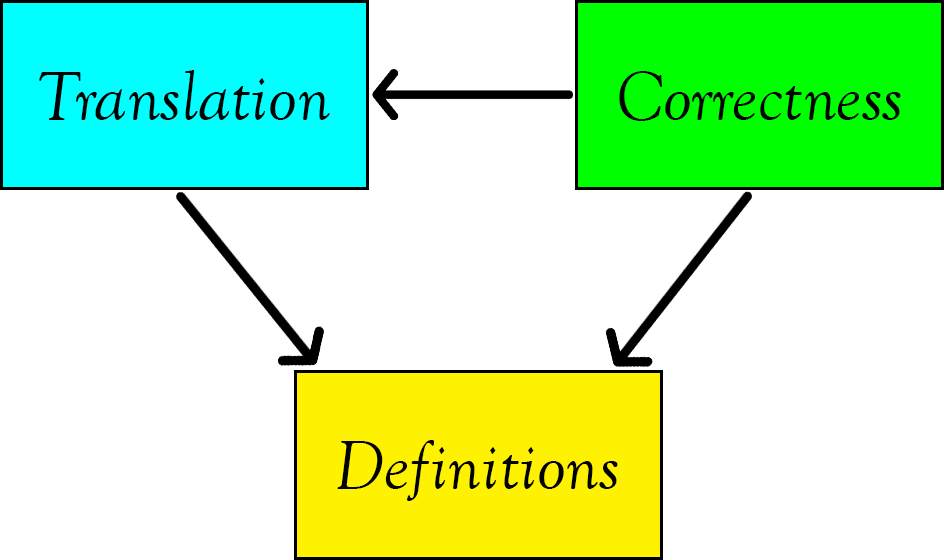
\includegraphics[width=.5\textwidth]{dependency} \end{center}

\par Readers are recommended to start with \textbf{Parsing-Regular-Expressions-in-Agda.agda}
,which is the index file of our formalisation. Now, let us look into each of the agda files. 

\begin{center}
\begin{longtable}{| p{5.2cm} | p{8.3cm} |}
\hline
\textbf{Parsing-Regular-Expressions-in-Agda.agda} & is the index
file of the Agda formalisation which imports all the other agda
files. Once this file has been compiled, all the other files will have been compiled as
well. \\ \hline 
\textbf{Subset.agda} & contains the definition and operations of subset. \\
  \hline
\textbf{../DecidableSubset.agda} & contains the definition and operations
                              of decidable subset. \\ \hline
\textbf{../VectorRep.agda} & contains the vector representation of sets. \\
  \hline
\textbf{Language.agda} & contains the definition and operations of language. \\
  \hline 
\textbf{RegularExpression.agda} & contains the definition of regular expression
                         and regular language. \\ \hline
\textbf{eNFA.agda} & contains the definition, operations and properties of
       \(\epsilon\)-NFA. \\ \hline
\textbf{NFA.agda} & contains the definition, operations and properties of
       NFA. \\ \hline
\textbf{DFA.agda} & contains the definition, operations and properties of
       DFA. \\ \hline
\textbf{MinimalDFA.agda} & contains the definition of minimal DFA. \\
  \hline 
\textbf{State.agda} & contains the state construction algorithm for
                      translating regular expressions to
                      \(\epsilon\)-NFA. \\ \hline
\textbf{Quotient.agda} & contains the quotient set construction
                         function for translating DFA to MDFA. \\
  \hline 
\textbf{RelationTable.agda} & contains the matrix representation of
                              a binary relation. This file is not
                              completed and thus it is not used in any
                              other files. \\ \hline
\textbf{Translation.agda} & is the index file of all the translation
                       algorithms. \\ \hline
\textbf{../RegExp-eNFA.agda} & contains the translation function
                                   \textbf{regexTo\(\epsilon\)-NFA} from regular
                                   expressions to \(\epsilon\)-NFA. \\
  \hline
\textbf{../eNFA-NFA.agda} & contains the translation function
                                   \textbf{remove-\(\epsilon\)-step}
                                from \(\epsilon\)-NFA to NFA. \\
                                \hline
\textbf{../NFA-DFA.agda} & contains the translation function
                                   \textbf{powerset-construction}
                                from NFA to DFA. \\
                                \hline
\textbf{../DFA-MDFA.agda} & contains the translation function
                                   \textbf{minimise}
                                from DFA to MDFA. \\
                                \hline
\textbf{../TableFillingAlgorithm.agda} & contains the algorithm
that computes the relation of distinguishable states. This file is not
completed and thus it is not used in any other files. \\
                                \hline
\textbf{Correctness.agda} & is the index file of all the correctness
                       proofs. \\ \hline
\textbf{../RegExp-eNFA.agda} & contains the proof that \(\forall
e\in RegExp.\ L(e) = L(regexTo\epsilon\)-NFA \(e)\). \\ \hline
\textbf{../../Epsilon-lemmas.agda} & contains the
\(\epsilon\) case of the above proof. \\ \hline
\textbf{../../Singleton-lemmas.agda} & contains the
\(\sigma\ a\) case of the above proof. \\ \hline
\textbf{../../Union-lemmas.agda} & contains the
union case of the above proof. \\ \hline
\textbf{../../Concatenation-lemmas.agda} & contains the
concatenation case of the above proof. \\ \hline
\textbf{../../KleenStar-lemmas.agda} & contains the
kleen star case of the above proof. \\ \hline
\textbf{../eNFA-NFA.agda} & contains the proof that \(\forall
enfa\in \epsilon\)-NFA\(.\ L(enfa) = L(remove\hyphen\epsilon\hyphen
step\ enfa)\). \\ \hline
\textbf{../NFA-DFA.agda} & contains the proof that \(\forall
nfa\in\)NFA\(.\ L(nfa) = L(powerset\hyphen construction\ nfa)\). \\ \hline
\textbf{../DFA-MDFA.agda} & contains the proof that \(\forall
dfa\in\)DFA\(.\ L(dfa) = L(minimise\ dfa)\). \\ \hline
\textbf{RegExp-Decidability.agda} & contains the proof of the
decidability of regular expressions. \\ \hline
\textbf{Example.agda} & contains an example on the recognition of a
string by a regular expression. \\ \hline
\textbf{Util.agda} & contains miscellaneous definitions and proofs
such as decidable equality. \\ \hline
\end{longtable}
\end{center}

\par We have also generated html files from the agda files. They are located in the \textbf{web} directory. Readers are
recommended to read the html files as it is much more
convenient. Similarly, readers can start with the
\textbf{Parsing-Regular-Expressions-in-Agda.html} which contains all
the links to other files. 

\section{Further Extensions}
\par In this section, we will discuss two possible extensions to
our project: 1) Myhill-Nerode Theorem and 2) Pumping Lemma. In these two
theorems, they both use the translation of regular expressions to DFA
in their arguments. Therefore, they can be built on top of our
formalisation. 


\subsection{Myhill-Nerode Theorem}
\par Given a language \(L\), and a pair of
strings \(u\) and \(v\), we define a relation \(R_L\) on strings such
that \(u R_L v\) if and only if for any string \(z\), \(uz \in L
\Leftrightarrow vz \in L\). The relation \(R_L\) is an equivalence
relation and thus it divides the set of strings into some equivalence
classes.
\par In general, the Myhill-Nerode Theorem states that a language
\(L\) is regular if and only if \(R_L\) has a finite number of
equivalence classes, and furthermore the number of states in the
minimal DFA translated from \(L\) is equal to the number of
equivalence classes in \(R_L\). The theorem is often used to prove a
language to be regular. 

\par In the proof, if \(L\) is a regular language, then a DFA is
translated from \(L\) to prove that \(R_L\) has finite equivalence classes. For the opposite direction, suppose \(R_L\)
has finite equivalence classes, then a DFA is also constructed from
the relation. By proving the DFA recognises \(L\), \(L\) is proved to
be regular. Therefore, the theorem can
be proved under the environment of our formalisation as we have
already formalised the translation from regular languages to DFA and its correctness proof. 


\subsection{Pumping Lemma (for regular languages)}
\par In general, the
Pumping Lemma states that if \(L\) is a regular language, then there
must exist an integer \(n \geq 1\) depending on \(L\) such that every
string \(w \in L\) of length at least \(n\) can be divided into three
sub-strings, i.e. \(w = xyz\) where
\begin{enumerate}[nolistsep]
  \item \(|y| \geq 1\);
  \item \(|xy| \leq n\);
  \item for all \(i \geq 0\), \(xy^iz \in L\).
\end{enumerate}
\par \(y\) is the sub-string that can be pumped (removed or repeated
any number of times) and the result string is always in \(L\). The
lemma is often used to prove a language to be non-regular. In the proof, a DFA is constructed from \(L\) to prove that there
must exist some loops in the path of \(w\). Therefore, it can be
proved by using our formalisation. 

\section{Evaluation}

\subsection{Correctness and Readability}
\par According to Geuvers \cite{geuvers2009}, a proof has two major roles: 1)
to convince the readers that a statement is correct and 2) to expain
why a statement is correct. The first role requires the proof to be
convincing. The second role requires the proof to be able to give an
intuition of why the statement is correct. In the paragraphs below, we
will discuss these two criteria. 

\paragraph{Correctness} Traditionally, when a mathematician submits
the proof of his/her concepts, a group of other mathematicians will
evaluate and check the correctness of the proof. Alternatively, if we
formalise the proof in a proof assistant, the proof will be checked
automatically by the compiler. The only difference is that we are now
relying on the compiler and the machine that runs the compile rather
than the group of mathematicians. Therefore, if the compiler and the
machine works properly, then any formalised proof that
can be compiled without errors are said to be correct. In our case, we
have the type checker and the termination checker in Agda to serve the
purpose. Furthermore, a proof is consist of smaller reasoning
steps. We can say that the a proof is correct if and only if all the
reasoning steps within the proof
are correct. When writing proofs in paper, we usually omit the proofs of
some obvious lemmas and this sometime leads to mistakes. However, in
Agda, we have to provide the proofs
of every lemma we have used explicitly. Therefore, the correctness of
an Agda proof always depend on the correctness of the smaller
reasoning steps that it contains. 

\paragraph{Readability} The second purpose of a proof is to explain why
a certain statement is correct. Let us consider the following code
snippet extracted from \textbf{Correctness/RegExp-eNFA.agda}. 

\begin{center} 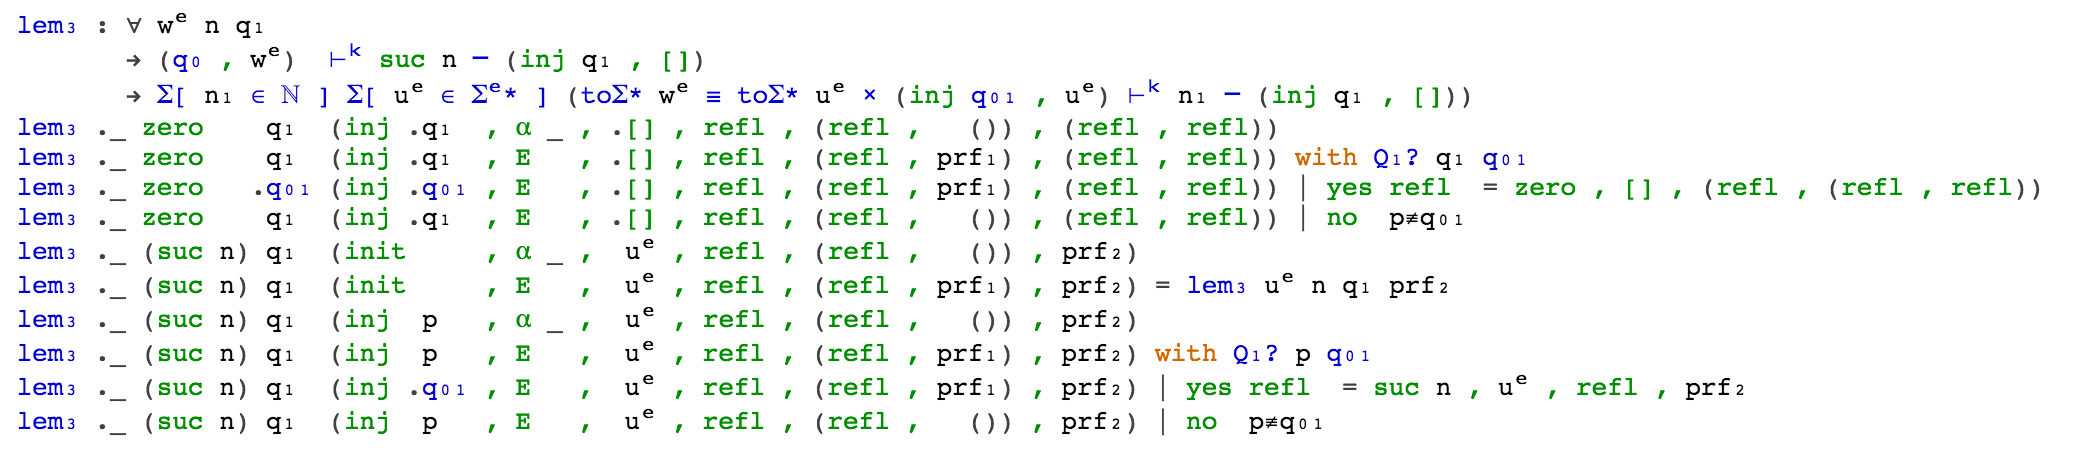
\includegraphics[width=\textwidth]{code} \end{center}

\par The above code is a proof that if \mb{w^e} can take \mb{q_0} to
another state \mb{inj\ q_1} in an \(\epsilon\)-NFA translated from a
regular expression \mb{e^*}, then there exists a number \mb{n_1} and
an \(\epsilon\)-string \mb{u^e} that will take \mb{inj\ q_{01}} to \mb{inj\ q_1} where
\mb{q_{01}} is the start state of \mb{e} and \mb{q_1} is a state in
\mb{e}. There are several techniques used in the proof including 
induction on natural numbers and case analysis of state comparison. However, by
just looking at the function body, we can hardly understand the
proving process. In conclusion, a computer proof is very inadequte on
this purpose and thus we still need to outline the concept of the proof using natural language. 


\subsection{Different choices of representations}
\par When writing computer proofs, we are usually required to
provide a concrete representation for abstract mathematical
objects. The consequence is that different represenations will lead to different
formalisations of the theorems and thus contribute to the
easiness or difficulty in completing the proofs. In our project, we have
made several decisions over the representations of different objects. In the
following parts, we will discuss their consequences. 

\paragraph{The set of states (Q) and its subsets} As we mentioned in section 3, Firsov and Uustalu
\cite{firsov2013} represented the set of states \mb{Q} and its subsets
as column matrices. However, this definition looks unnatural compare
to the actual mathematical definition. Therefore, at the beginning of
our project, we tried to avoid the vector representation. In our
apprach, the set of states are represented as a data type in Agda, i.e. \mb{Q : Set}, and its
subsets are represented as unary functions on \mb{Q}, i.e. \mb{DecSubset\ A = A \to
  Bool}. 

\par Our definiton allows us to finish the proofs in
\textbf{Correctness/RegExp-eNFA.agda} without having to
manipulate matrices. The proofs look much more natural compare to that in
\cite{firsov2013}. However, the problem arises when we need to iterate the set of states
and its subsets when we are computing the
\(\epsilon\)-closure. However, by using this definition, there is no possible way
for us to iterate the sets. Therefore, we still need to include \mb{It} -- a
vector containing all the states in \mb{Q}, in the definition of automata. By
using \mb{It}, we can iterate the subsets of \mb{Q} by applying the
function \mb{Q \to Bool} to all the elements in \mb{It}. Note that the
vector \mb{It} is actually the vector representation of the set of
states and therefore, we cannot avoid it. 

\paragraph{The language accepted by regular expression} At first, we
defined the language accepted by regular expression as a decidable
subset, i.e. \mb{L^R : RegExp \to (\Sigma^* \to Bool)}. 

\subsection{Problems arise}
\par Let us recall the definition of reachable states in
\textbf{Translation/DFA-MDFA.agda}. 

\begin{center} 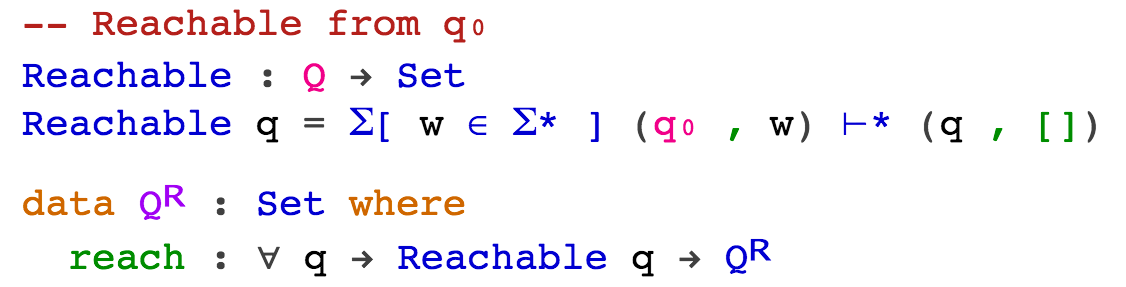
\includegraphics[width=.6\textwidth]{reach} \end{center}

\par We say that a state \mb{q} is reachable if and
only if there exists a string \mb{w} that can take \mb{q_0} to
\mb{q}. Therefore, the set \mb{Q^R} should contains all and only the
reachable states in \mb{Q}. However, there may exsist more than one
reachability proof for a single state. This implies that there may be
more than one element in \mb{Q^R} having the same state. Therefore, \mb{Q^R}
may be larger than the original set \mb{Q} or even worse, it may be
infinite. This leads to a problem when we construct a
new DFA using \mb{Q^R} as the set of states. If \mb{Q^R} is
infinite, then we have no possible way to iterate the set in 
quotient construction. Even if the set \mb{Q^R} is finite, the
computational cost will be much higher. This is also one of the
reasons why we cannot finish the quotient construction. However,
surprisingly, this has no effects to the proof of \mb{L(DFA) =
  L(MDFA)} because we can provide an equality relation of states in
the record \mb{DFA}. In the translation from DFA to MDFA, we defined
the equality relation as follow: any two states in \mb{Q^R} are equal if and only
if the input states are equal. Therefore, two elements with same state
but different reachability proofs are considered to be the same state
in the new DFA. 

\par One possible way to solve the problem is to re-define the
reachability of a state such that any reachable state will have a
unique reachability proof. For example, we can sort the reachablility
proofs according to alphabetical order of the string \mb{w} and choose the proof
with shortest string as the representative. This also requires a proof that
the chosen proof is unique. Another solution is to use
homotopy type to declare the set \mb{Q^R}. This type allows us to
group different reachability proofs into a single element such that
every state will only appear once in \mb{Q^R}. 


\section{Conclusion}
\par In our project, the translation from regular expressions to DFA
and its correctness proof were formalised in Agda. However, the parts
related to the translation from DFA to MDFA were not completed. The
parts include the Table-filling algorithm that is used when
constructing the quotient set and the correctness of the
algorithm. However, the framework of the those parts was already formalised
in Agda; therefore, it is possible to complete the parts by filling in
the details. Therefore, it is still feasible to formalise the translation in
Type Theory. 

\nocite{*}
\addcontentsline{toc}{chapter}{Bibliography}
\bibliographystyle{plain}
\bibliography{references}


\begin{appendices}
\chapter{File description}

\par There are two directories in the .zip file: 1) \textbf{Code} and 2)
\textbf{web}. The \textbf{Code} directory contains all the
\textbf{.agda} files. In order to compile these files, first install
Agda by following the instructions stated in
\href{http://wiki.portal.chalmers.se/agda/pmwiki.php?n=Main.Download}{The
Agda Wiki}. Then open
\textbf{Parsing-Regular-Expressions-in-Agda.agda} with the IDE
recommended by the website. Press Ctrl-c Ctrl-l to compile the
file. The \textbf{Parsing-Regular-Expressions-in-Agda.agda} file is an
index file that imports all other agda files. Once this file has been
compiled, the other Agda files will have been compiled as well. 
\par The \textbf{web} directory contains all the html files generated
from the agda files. Readers are recommended to read the html files
instead of the agda files especially for those who do not have Agda
installed. The \textbf{Parsing-Regular-Expressions-in-Agda.html} is
the index file that contains the links to all other html files. 
\end{appendices}

\end{document}